\chapter{Modeling UASs for Role Fusion and Human Machine Interface Optimization}

\noindent TJ Gledhill, Eric Mercer and Michael A. Goodrich. Modeling UASs for Role Fusion and Human Machine Interface Optimization. In Proceedings of IEEE International Conference on Systems, Man, and Cybernetics, Manchester, England, 2013.

\begin{abstract}
Currently, a single Unmanned Aerial System (UAS) requires several humans managing different aspects of the problem. Human roles often include vehicle operators, payload experts, and mission managers~\cite{goodrich2008supporting,MurphyStoverPrattGriffin2006,Cummings2007}. As a step toward reducing the number of humans required, it is desirable to reduce operator workload through effective distributed control, augmented autonomy, and intelligent user interfaces. Reliably doing this requires various roles in the system to be modeled. These roles naturally include the roles of the humans, but they also include roles delegated to autonomy and software decision-making algorithms, meaning the GUI and the unmanned aerial vehicle. This paper presents a conceptual model which models the roles of complex systems as a collection of actors, running in parallel.  Results from applying this model to the UAS-enabled Wilderness Search and Rescue (WiSAR) domain indicate (a)~it is possible to model the entire WiSAR system at varying degrees of abstraction (b)~that building and evaluating the model provides insight into the best practices of WiSAR teams and (c)~a way to model human machine interactions that works directly with the Java Pathfinder model checker to detect errors.

%can provide new insight into human machine interactions through role.   UAS-enabled Wilderness Search and Rescue (WiSAR) %as a collection of roles running in parallel.   as well as an encoding of this model in Java. This yields a precise formalization of %the individual WiSAR roles and allows behavior of the roles to be model-checked by
%Java Pathfinder to establish bounds and trends in the models. Results from the modeling activity and model-checking in Java %Pathfinder indicate (a)~that it is necessary to clearly identify an appropriate level of modeling abstraction and (b)~that building %and evaluating the model provide insight into the best practices for real and UAS-enabled WiSAR teams.
\end{abstract}

\section{Introduction}

Most existing Unmanned Aerial Systems (UASs) require two or more human operators\cite{goodrich2008supporting,MurphyStoverPrattGriffin2006}. Standard UAS practice is to have one human to control the aerial vehicle and another to control the camera or other payloads. In addition to this a third human is often responsible for overseeing task completion and interfacing with the command structure. Although some argue persuasively that this is a desirable organization~\cite{MurphyBurke2010}, there is considerable interest in reducing the required number of humans and reducing human workload using improved autonomy and enhanced user interfaces~\cite{Cummings2007,MitchellCummings2005,goodrich2010fanout}.

The broad research context driving this paper takes a multistep approach: (a)~model the roles for a specific UAS and a well-defined set of tasks, (b)~delimit assumptions and abstractions used in the model, (c)~verify properties of the model, (d)~use the model to explore ways of combining roles in such a way that operator workload and the number of humans is minimized, and (e)~design vehicle autonomy and user interface support to allow a real UAS team to operate more efficiently. The focus of this
paper is on the important lessons learned in the first two steps.

The modeling used in this paper could be applied to a number of tasks, but we focus on Wilderness Search and Rescue for two reasons. First, the authors have done prior work on UAS-enabled Wilderness Search and Rescue (WiSAR)~\cite{goodrich2009towards}; and second, there is a host of modeling information about how WiSAR is currently performed~\cite{adams2009cognitive}. The UAS-enabled WiSAR systems produced by this research requires three humans, two GUIs, and a single UAV.

To gain insight into WiSAR we have chosen to model the system as a group of directed role graphs (DiRGs).  Each human, GUI, and UAV represent a DiRG, allowing evaluation of potential conflicts between and opportunities for unification of the various roles.  These DiRGs are referred to as \emph{Actors} in the models below.  

Modeling is essentially a process of abstraction, choosing which elements of a system are essential and which are not~\cite{Box1976}. Since one of the goals of this paper is to use model-checking to evaluate models, we choose a model class that is simple enough that it allows us to clearly delineate between what is modeled and what is not. Thus, we use DiRGs, which can be expressed as Mealy state machines, to model different WiSAR roles. These models explicitly encode key aspects of the various actors, and collectively form a group of Mealy machines that run in parallel. The model is encoded in Java using a custom set of interfaces designed to simulate a discrete time environment, facilitate input/output between roles, and provide non-deterministic event handling.  

Model checking is performed using Java Pathfinder (JPF).  This is convenient because JPF runs the model checking on the compiled Java code generated by the modeling exercise.

The results of this modeling exercise indicate (a)~it is possible to model the entire WiSAR system using varying degrees of abstraction and (b)~that building and evaluating the model provides insight into the best practices of WiSAR teams and (c)~a way to model human machine interactions that works directly with the Java Pathfinder model checker to detect errors.

%Given the models we can use model checking to verify the model and identify bounds and trends in the models. The model %checking is performed using Java Pathfinder (JPF), which is convenient
%because JPF runs the model checking on the compiled Java code.

\section{Related Work}
NASA Ames Research Center (NASA ARC) is using Brahms, a complex and robust language, to model interactions
between operators and their aerial equipment~\cite{rungta2013aviation}. To study the Uberlingen collision, an in air collision of two commercial passenger planes, Rungta and her colleagues produced a model entirely in the Brahms language. This model correctly predicts the collision and also reveals some of the difficulties intrinsic to this type of system.

One critical aspect of NASA ARC�s work carries over into our own: variable task duration~\cite{hunter2013a}.  Task duration directly influences whether the situation ends safely, barely avoids a crash, or crashes.  The biggest advantage Brahms has over Java comes from its strict grammar. However, Brahms must be translated into Java before using JPF, a step we avoid by implementing our model in Java directly.

Bolton and Bass used the Enhanced Operator Function Model (EOFM) language to create a model consisting of the Air Traffic Controller, the pilot flying the plane, and the pilot monitoring the equipment, as well as the interfaces they used~\cite{bolton2009enhanced}. As they increased the number of allowable miscommunications, their system had an exponential increase of errors. EOFM facilitates the division of goals into multiple levels of activities. These activities can then be broken into atomic actions~\cite{bolton2013evaluating}. The main difference between this model and our own is that EOFM is expressed in XML while ours is expressed in Java.  This allows us to perform model checking directly using JPF.

Wilderness Search and Rescue is primarily concerned with finding people who have become lost in rugged terrain. Research has shown that UASs could potentially be used to facilitate this work. Goodrich et al. tested the effectiveness of these types of operations~\cite{GoodrichMorse2008}. A key outcome of these field tests is the speculation that effectiveness could be enhanced if the roles of the UAV operator and video operator were combined.

In prior work, a goal-directed task analysis, a work domain analysis, and a control task analysis were performed.~\cite{adams2009cognitive}.  These analyses modeled WiSAR as a collection of goals, work domains, and tasks.  While these studies proved valuable for understanding the WiSAR processes they were less helpful in suggesting improvements to the WiSAR processes. Indeed, the limitations of such tools for informing the design of technology to support existing processes has lead to new methods for performing such analyses~\cite{humphrey2009information}; the work in this paper complements such work, using model-checking to perform analyses on problems that do not lend themselves to answers using other approaches.

\section{WiSAR UAS Domain}

Wilderness search and rescue often occurs in
remote, varying, and dangerous terrains. According to~\cite{setnicka1980}, there are four core elements of a WiSAR operation: {\it Locate}, {\it Reach}, {\it Stabilize}, and {\it Evacuate}.  The WiSAR UAS operates within this first element so it is the focus of this paper.

%\begin{figure}[h]
%\begin{center}
%\begin{math}
%Locate \Rightarrow Reach \Rightarrow Stabilize \Rightarrow Evacuate
%\end{math}
%\end{center}
%\caption{Core SAR Elements}
%\label{fig:sar}
%\end{figure}

During the {\it Locate} element, the incident commander (IC) develops a strategy to obtain information. This strategy makes use of the available tactics to obtain this information. The WiSAR UAS is one of the tactics that the IC may choose to use. A WiSAR UAS technical search team consists of three humans: Mission Manager, Vehicle Operator, and Video Operator. These constitute the three human roles in the team. Supporting these human roles are two intelligent user interfaces, the Vehicle Operator GUI and the Video Operator GUI; these constitute two other roles that must be modeled. The final role is the aerial vehicle itself, which is equipped with sensors and controllers that enable it to make decisions.
Since the WiSAR UAS technical search team must coordinate its efforts with other members of the search team via the IC, we embed the five UAS roles within a Parent Search model. The parent search model represents the entire
command structure for the search and rescue operation.

In the next section, we model the WiSAR roles and the interactions between these roles. Naturally, these roles will need to take input from the environment, so we present a simple model of the environment that emphasizes the key environmental elements, probabilistic events and varying task durations. Note that this model of the environment exists at a higher level of abstraction than what is typically considered an environment model in literature; typical models tend to focus on environmental realism, encoding things like terrain, wind, etc, but our model emphasizes events that affect the behavior of the WiSAR roles.

\section{Conceptual Model}
We have chosen to conceptualize the WiSAR UAS as a group of DiRGs.  A DiRG represents a sequence of tasks for a single role.   By conceptualizing WiSAR as a collection of DiRGs running in parallel we hope to gain more insight into the WiSAR processes with a goal of improving these processes.  In prior work, a goal-directed task analysis, a work domain analysis, and a control task analysis were performed.~\cite{adams2009cognitive}.  These analyses modeled WiSAR as a collection of goals, work domains, and tasks.  While these studies proved valuable for understanding the WiSAR processes they were less helpful in suggesting improvements to the WiSAR processes.  Indeed, the limitations of such tools for informing the design of technology to support existing processes occurs because they discover conditions which may result in problems rather than discovering system problems themselves.  Performing system-level task modeling, such as we are, is capable of discovering such problems~\cite{bolton2013litreview}.     

While we are using this technique to find such problems we expand on it in several ways.  First, this technique is most commonly used for analyzing a single human using an interface.  Our models involve a team of humans simultaneously using multiple interfaces which naturally increases the state space of the model, decreasing scalability.  Second, we are using this technique to analyze the workload of the system.  Our goal is the combining of human roles and interfaces.  We hope to gain insight into decreasing the system workload, and possibly combining roles, by establishing metrics associated with the task model and model simulation.  These metrics can then be used to determine if changes to the model represent a decrease in operator workload.

As is common when modeling human-automation interaction we have decided to model the DiRGs usings Mealy state machines~\cite{bolton2013litreview}  This allows us to abstract the different WiSAR roles into individual state machines that we call Actors.  Actors do not correspond to a single aspect of the WiSAR domain, anything can be an Actor, thus providing the freedom to flexibly model as many aspects of the domain as necessary and at various levels of resolution.  This freedom is important and represents our primary method of reducing the state space to manage scalability.  Actors transition between states by receiving  inputs generated by other Actors and Events.  Events are also modeled as Mealy machines whose transitions are triggered by a combination of simulation and Actor inputs.  Because Actors and Events may receive input from other Actors and Events the combination of their transition matrices define the wiring of the different DiRGs.  A single wire is when an output from one Actor is an input on another Actor.  This implies that the set of all inputs is the same as the set of all outputs, however, in practice we do not treat these sets as the same since unhandled input represents transitions returning to the current state.  We ignore these looping transitions except when their behavior tells us something interesting.

Formally, the models are the following mathematical structures:
 \begin{equation}
 	Actor = (S, s_0, \Sigma_A \cup \Sigma_, \Lambda_A, T)
 \label{eq:mealymachine}
 \end{equation}

 \begin{equation}
	Event = (S, S_0, \Sigma_{A} \cup \Sigma_{S}, \Lambda_{A}, T)
 \label{eq:mealymachine}
\end{equation}

\begin{equation}
	T : S \times \Sigma \Rightarrow S \times \Lambda_A
 \label{eq:mealymachine}
\end{equation}


where $S$ is a set of states, $s_0$ the start state,  $\Sigma_{A}$ the set of all Actor inputs, $\Sigma_{S}$ the set of all Simulator inputs, $\Lambda_{A}$ the set of all Actor outputs, and $T$ a transition matrix which specifies the outputs for any state transition.  $T$ may have multiple inputs and multiple outputs.

At this point our conceptual model is implementation agnostic.  Indeed, the abstraction allows us to group Actors, break Actors into sub-Actors, and use Actors to validate specific behaviors.  The model also allows for complex transitions between Actor states and the ability to enter normally unreachable state spaces using Events.  The model is also easily adapted to code which can be verified using model checking tools such as Java Pathfinder (JPF) which we will show in the following sections.

\section{Simulating the WiSAR UAS}
Real WiSAR environments and UAV dynamics are complex so full models of the environment and UAV can also become extremely complex.  However, many of the complexities are not relevant to the decisions made by the various WiSAR actors.  Consequently, we propose a model that "abstracts away" many unessential details and encodes key aspects of the environment.  In order to simulate critical aspects of the WiSAR UAS model it is necessary to represent communication between Actors, concurrency, and task duration, concepts which are outside the scope of a standard state machine. To do this we constructed a basic simulation framework.  The simulation framework is encapsulated into a single Java class, called {\em Simulator}. This section discusses the key components of this simulation framework.

\subsection{Core Simulator Objects}
The Simulator is made up of the following objects:  Team, Actors, Events, States, Transitions, and Unique Data Objects (UDO).  We organize these objects in the following way.  A Team is a wrapper class representing the entire model which contains a collection of Actors, Events, and shared UDOs.  Each Actor contains a set of private States.  Each of these States contains a set of Transitions.  Each Transition contains a set of input UDOs, a set of output UDOs, the outgoing Actor State, and a reference to the Actors current State.  This structure is convenient because it naturally encapsulates the different aspects of a Mealy machine.  

Each UDO represents a unique piece of data, input or output, and is flagged as active or inactive.  A UDO is temporarily set to active after it is sent as output.  Each Transition can easily determine if it is possible by checking to see that all of its input UDOs are active.  Each State can then return a list of possible transitions.  An Actor evaluates the list of possible Transitions to determine how it should transition.  If it is empty then the Actor does not transition, otherwise the Actor chooses a single Transition to occur.  An Actor chooses a Transition at the Simulators request.  The Simulator tracks when this Transition should occur, at which point the Transition will set each output UDO to active and change the Actors current state to the Transitions outgoing State.  Because the UDOs must exist before Actors can be initialized we have created the Team class.  The Team class wraps all of the Actors, Events, and UDOs into single entity.  This class first initializes each UDO, afterwards each Actor and Event is initialized with a list of input and output UDO references which it will use in its transitions.  This structure offers a few benefits.  Code wise it allows us to simulate the transfer of data without actually transferring data which drastically simplifies the code.  It also forces us to explicitly define our model wiring in two places, first at the Team level and second at the Actor Transition level as mentioned above.  Although the Transition set of inputs is not limited to the set of global UDOs we can still compare the set of global inputs and outputs an Actor receives with the set of inputs and outputs defined by its transitions.  Through this we can validate that the set of Actor transitions is complete, as defined in our Team, which is an important step in validating the model.  A simple example of the initialization of the Team and its components is shown in the following example:

\begin{verbatim}
Team {
    UDO A1Output = new UDO()
    UDO E1Output = new UDO()

    UDO Inputs[] = [E1Output]
    UDO Outputs[] = [A1Output]
    Actor A1 = new Actor(Inputs, Outputs)

    UDO Inputs[] = [A1Output]
    Actor A2 = new Actor(Inputs, [])

    UDO Outputs[] = [E1Output]
    Event E1 = new Event([], Outputs)
}

A1(Inputs, Outputs) {
    State S1 = new State()
    State S2 = new State()

    S1.addTransition(this, 
        Inputs.E1_Output, 
        Outputs.A1Output, 
        S2)
}

A2(Inputs, Outputs) {
    State S1 = new State()
    State S2 = new State()

    S1.addTransition(this, 
         Inputs.A1Output, 
         null, 
         S2)
}

E1(Inputs, Outputs) {
    State S1 = new State()
    State S2 = new State()

    S1.addTransition(this,
        null, 
        Outputs.E1Output, 
        S2)
}
\end{verbatim} 

While this is only a basic example it clearly shows how the models have been implemented as code.  The example also illustrates the Event class.  Events differ from Actors in that Event transitions require an express command from the Simulator before processing.  This allows the Simulator to non-deterministically trigger events which, when run in JPF, can be setup to process events at different intervals or when the system changes state.  From this we can determine the effects events have on the system in a very robust manner.

\subsection{Communication Between Actors}
To simulate a team of Actors working together it is necessary to establish a communication medium within the model and simulation which can represent the different forms of communication.  In the model this communication medium is represented as inputs, outputs, and transitions.  

Our initial attempts to simulate this communication resulted in a PostOffice class attached to the Simulator.  Actors sent data along with the name of the recipient to the PostOffice.  Actors could then retrieve their input from the PostOffice, much the way PO boxes work.  Actors also had the ability to make certain output observable through the PostOffice.  This meant that an Actor could place data into the PostOffice for other Actors to observe, a public PO box.  When we added sub-Actors to the model code it became necessary to allow Actors and sub-Actors to share both private and public PO boxes.  It was also necessary to store current and future output separately to achieve concurrency which we explain in the next section.  Although this achieved the desired goal the results were less than satisfactory.  In addition to the added complexity the design used implicit input and output connections making it much harder to validate that the code represented the desired model.

Our next iteration of the Simulator simplified this communication medium with the use of the previously defined UDOs.  By initializing these UDOs and passing them as references to the Actors and Events we greatly simplified inter-Actor communication.  This new design also requires explicit declarations for each UDO connection allowing us to validate the model code with the model and again with the transition matrixes.  The UDO is also capable of representing both direct and observable communications which naturally allow sub-Actors to link inputs with parents.  Indeed, Actor relationships are now irrelevant in regard to sharing input and output since Actors only depend on the status of the UDOs.  In the case where it does matter which Actor generated the output then a new UDO can be created representing that relationship thus preserving Actor independence through explicit connections.

The Team initialization example above demonstrates the use of UDOs.  The example
defines two UDOs, A1Output and E1Output.  Once defined these UDOs are passed
by reference to specific Actors and Events as inputs, explicitly defining the
connectivity implied by the UDOs.  The Actors use the UDO references for
constructing their transition matrices which results in the connecting of A2 to
A1 and A1 to E1.  If we desired to change our model and allow A2 to transition on E1Output the UDO would be added to the A2 input and A2 would declare a transition for that input resulting in the connectivity of A2 to E1.

\subsection{Simulating Time}
To simulate task duration the simulator uses the delta time algorithm.  Each Transition has a specified duration range defined by the Actor or Event.  The simulator has five different duration settings for choosing a value within a range: $MIN$, the minimum; $MAX$, the maximum; $MIN\_OR\_MAX$, a random choice between one of these settings; $MIN\_MEAN\_OR\_MAX$, another random choice..  When an Actor begins a Transition the Simulator chooses a duration, the value of that duration is then converted to the Simulator delta time.  Basically if a transition is to finish in 30 time steps but another Transition finishes at 25 time steps then the first Transition is placed after the second Transition and is given a count of 5 which means it happens 5 time steps after the prior Transition.  Thus as the simulation progresses time remains relative.

Slightly different from the use of transition durations is the notion of simulating Events.  The time range over which an Event may occur is often much larger than the ranges defined by tasks, also, Events are only possible in specific state spaces thus preventing us from predicting the available time range of the Event.  This prevents us from simulating Event timing in the same way as task durations because such large time ranges cannot be accurately represented with with only 2 to 3 choices and we cannot select a min, max, or mean if the range is unknown.  We solve this problem in two ways.  One method is to trigger the Event at regular time intervals while the Event is possible.  Depending on the interval size this can cause a dramatic increase in state space.  While this increases the possibility of exploring the possible effects an Event can generate on the system it offers no guarantees.  Another method for triggering Events is to trigger the Event on each state change within the system while the Event is possible.  This guarantees that the Event will be explored in each state space that is presented during the simulation, however, this is also likely dramatically increase the state space and is much more difficult to implement.  Since triggering an Event represents a transition within the Event it is included in the delta time algorithm used for progressing simulation time.

\subsection{The Simulation Loop}
It is now possible to describe the actual simulation.  After initialization we enter the simulation phase.  This phase is used to transition the Actors and trigger Events.  One challenge with transitioning the Actors is the need for concurrency.  The simulation must allow multiple Actors to transition without interfering with one another.  Previous versions of our Simulator placed each Actor within its own thread.  We found that threads complicate the conversion into JPF so instead we chose to use transactions.  In each transaction we allow each Actor to make the changes required by its transition.  These transitions only modify a temporary value on the UDOs.  After all transitions are completed we finish the transaction by moving each temporary UDO value into the actual value.  The entire simulation phase can be described thus:

\begin{verbatim}
Begin Transaction:
    Foreach Actor
        if ( Transition duration reached )
            Process Transition

    End Foreach
End Transaction

Process Transaction

Foreach Actor
    Transition = Get Next Transition
    If Transition is not null
        Convert Transition duration to delta time.
        Update necessary Actor delta times.
End Foreach
\end{verbatim}

When there are no longer any pending Transitions the loop ends and the simulation is terminated.


\begin{comment}
\section{Conceptual Model}
We have chosen to conceptualize the WiSAR UAS as a group of DiRGs.  A DiRG represents a sequence of state changes for a single role.   By conceptualizing WiSAR as a collection of DiRGs running in parallel we hope to gain more insight into the WiSAR processes with a goal of improving these processes.  In prior work, a goal-directed task analysis, a work domain analysis, and a control task analysis were performed.~\cite{Adams2008}.  These analyses modeled WiSAR as a collection of goals, work domains, and tasks.  While these studies proved valuable for understanding the WiSAR processes they were less helpful in suggesting improvements to the WiSAR processes. Indeed, the limitations of such tools for informing the design of technology to support existing processes has lead to new methods for performing such analyses~\cite{humphrey2009information}; the work in this paper complements such work, using model-checking to perform analyses on problems that do not lend themselves to answers using other approaches. 

This conceptual model uses Mealy state machines.  This allows us to abstract the different WiSAR roles into individual state machines that we call Actors.  Actor states do not correspond to a single aspect of the WiSAR domain, thus providing the freedom to flexibly model as many aspects of the domain as necessary and at various levels of resolution. Actors transition between states are triggered by inputs generated by Events and by other Actors.  Events are also modeled as Mealy machines whose transitions are triggered by a combination of simulator and Actor inputs.  

Formally, the models are the following mathematical structures:
 \begin{equation}
 	Actor = (S, S_0, \Sigma_A, \Lambda_A, T)
 \label{eq:mealymachine}
 \end{equation}
 \begin{equation}
	Event = (S, S_0, \Sigma_{A} \cup \Sigma_{S}, \Lambda_{A}, T)
 \label{eq:mealymachine}
\end{equation}

\begin{equation}
	T : S \times \Sigma \Rightarrow S \times \Lambda_A
 \label{eq:mealymachine}
\end{equation}
where $S$ is a set of states, $S_0$ the start state,  $\Sigma_{A}$ the set of all Actor inputs, $\Sigma_{S}$ the set of all Simulator inputs, $\Lambda_{A}$ the set of all Actor outputs, and $T$ a transition matrix which specifies the outputs for any state transition.

A benefit of this state machine-based conceptual model is the ability to convert the model into code. The coded model can be verified using model checking tools such as Java Pathfinder (JPF) to gain further insight into the model.  In the interest of space we will not describe the Java simulation framework developed for JPF model checking.


\section{Simulating the WiSAR UAS}
Real WiSAR environments and UAV dynamics are complex  so full models of the environment and UAV can also become extremely complex.  However, many of the complexities are not relevant to the decisions made by the various WiSAR actors.  Consequently, we propose a model that "abstracts away" many unessential details and encodes key events.  To do this we constructed a basic simulation framework.  The simulation framework is encapsulated into a single Java class, called {\em Simulator}. This section discusses the key components of this simulation framework.

In order to simulate critical aspects of the WiSAR UAS model it is necessary to model all of the different roles, interfaces, and objects in a simplified way that encodes the set of possible interactions.  We chose to do this using state machines. More precisely, we represent these elements using Mealy state machines because there is a clear correlation between states and actions that our Actors are undergoing. Also Mealy state machines are easily translated into code. We refer to these state machines as {\em actors}. Events are Mealy State machines that differ from actors in that they require input from the simulator as well as from at least one actor before they will change state. Formally, actors and events are modeled as Mealy machines
\begin{equation}
	Actor = (S, S_0, \Sigma_A, \Lambda_A, T)
\label{eq:mealymachine}
\end{equation}

\begin{equation}
	Event = (S, S_0, \Sigma_A \cup \Sigma_S, \Lambda_A, T)
\label{eq:mealymachine}
\end{equation}

\begin{equation}
	T : S \times \Sigma_A \Rightarrow S \times \Lambda_A
\label{eq:mealymachine2}
\end{equation},
where $S$ is a set of states, $S_0$ the start state,  $\Sigma_{A}$ the set of all Actor inputs, $\Sigma_{S}$ the set of all Simulator inputs, $\Lambda_{A}$ the set of all Actor outputs, and $T$ a transition matrix which specifies the outputs for any state transition.

The events encoded in the Mealy state machine represent asynchronous occurrences in the real world. We simulate the flow of these asynchronous events, and their consequences on the decisions of the actors, using sequential code that explicitly represents the passage of time. Simulating the passage of time provides a means whereby we can monitor the interactions between Actors in our model. Each action an Actor can take is assigned a range spanning the minimum and maximum time required to complete thereby inserting non-determinism into the system.

\subsection{Non-Determinism}

We control the level of non-determinism through the simulator with a DurationGenerator class.  This class has five different duration settings: $MIN$, the minimum; $MAX$, the maximum; $MIN\_OR\_MAX$, a random choice between one of these settings; $MIN\_MEAN\_OR\_MAX$, another random choice; and $RANDOM$, a completely random choice. In translation these settings reflect possible task durations: . The number of state spaces this produces can be seen in table~\cite{} in our results.

\subsection{Concurrency}

To help give the appearance of concurrency during the processing of a timestep we implemented an output storage and distribution class called PostOffice.  Output is sent to the PostOffice using these methods:
\begin{verbatim}
addOutput(IData data, String name);
addObservation(IData data,
    String actor_name);
\end{verbatim}

The PostOffice uses Actor names to deliver outputs.  The PostOffice keeps all output in a temporary hash map.  At the desired time the simulator will tell the PostOffice to make the temporary output current.  At this point the current output is destroyed and the temporary output is emptied into the current output. This prevents output received during the same processing step from being received before its due time.  An Actor may also post observations which are output that must be requested by other Actors. Actors pull input and observations from the simulator using these methods:
\begin{verbatim}
ArrayList<IData> getInput(String);
ArrayList<IData> getObservations(String);
\end{verbatim}
The PostOffice also has the ability to link output and observations for multiple actors by mapping Actor names to one another.  This feature was added to allow sub-actors to automatically share input with parent Actors and to allow observation of a parent Actor to return the observations of all of its children.

\subsection{Actors and Event Interfaces}

Each Actor implements the IActor interface with the methods: processNextState and processInputs. The processNextState moves the actor into its next state, generating outputs and setting the next state to a default value and duration. The processInputs method then looks at its inputs and determines what the next state should be and when it should occur. This method also generates additional outputs.
\begin{verbatim}
	public interface IActor {
		    public int nextStateTime();
		    public void processNextState();
		    public void processInputs();
		    public String name();

	}
\end{verbatim}

Each Event implements the IEvent interface. The IEvent interface is fairly similar to the IActor interface except it has the method getCount. This makes it possible to insert multiple events of the same type without having to instantiate entirely new objects. Events are also given higher priority than Actors ensuring that all applicable events execute prior to any actors on a given time-step; this is necessary to enable our sequential model to properly simulate asynchronous events in the world.
\begin{verbatim}
	public interface IEvent {
	    public int getNextTime();
	    public void processNextState();
	    public void processInputs();
	    public int getCount();
	}
\end{verbatim}

\subsection{Event Flow}

Each Actor has a method getNextStateTime. This returns the global time-step when the actor will change state.  This assumes that everything in the system requires at least one time step to complete, and is a reasonable way of simulating asynchronous event flow provided that the time step is small. The simulator takes the minimum value of all the nextStateTimes and advances the global clock to that time.  If however the time outputted is 0 then the simulator treats that as a signal that the model is done processing and terminates. This eliminates unnecessary processing by ensuring the simulator only processes time steps when the system is changing.

\begin{figure}
\centering
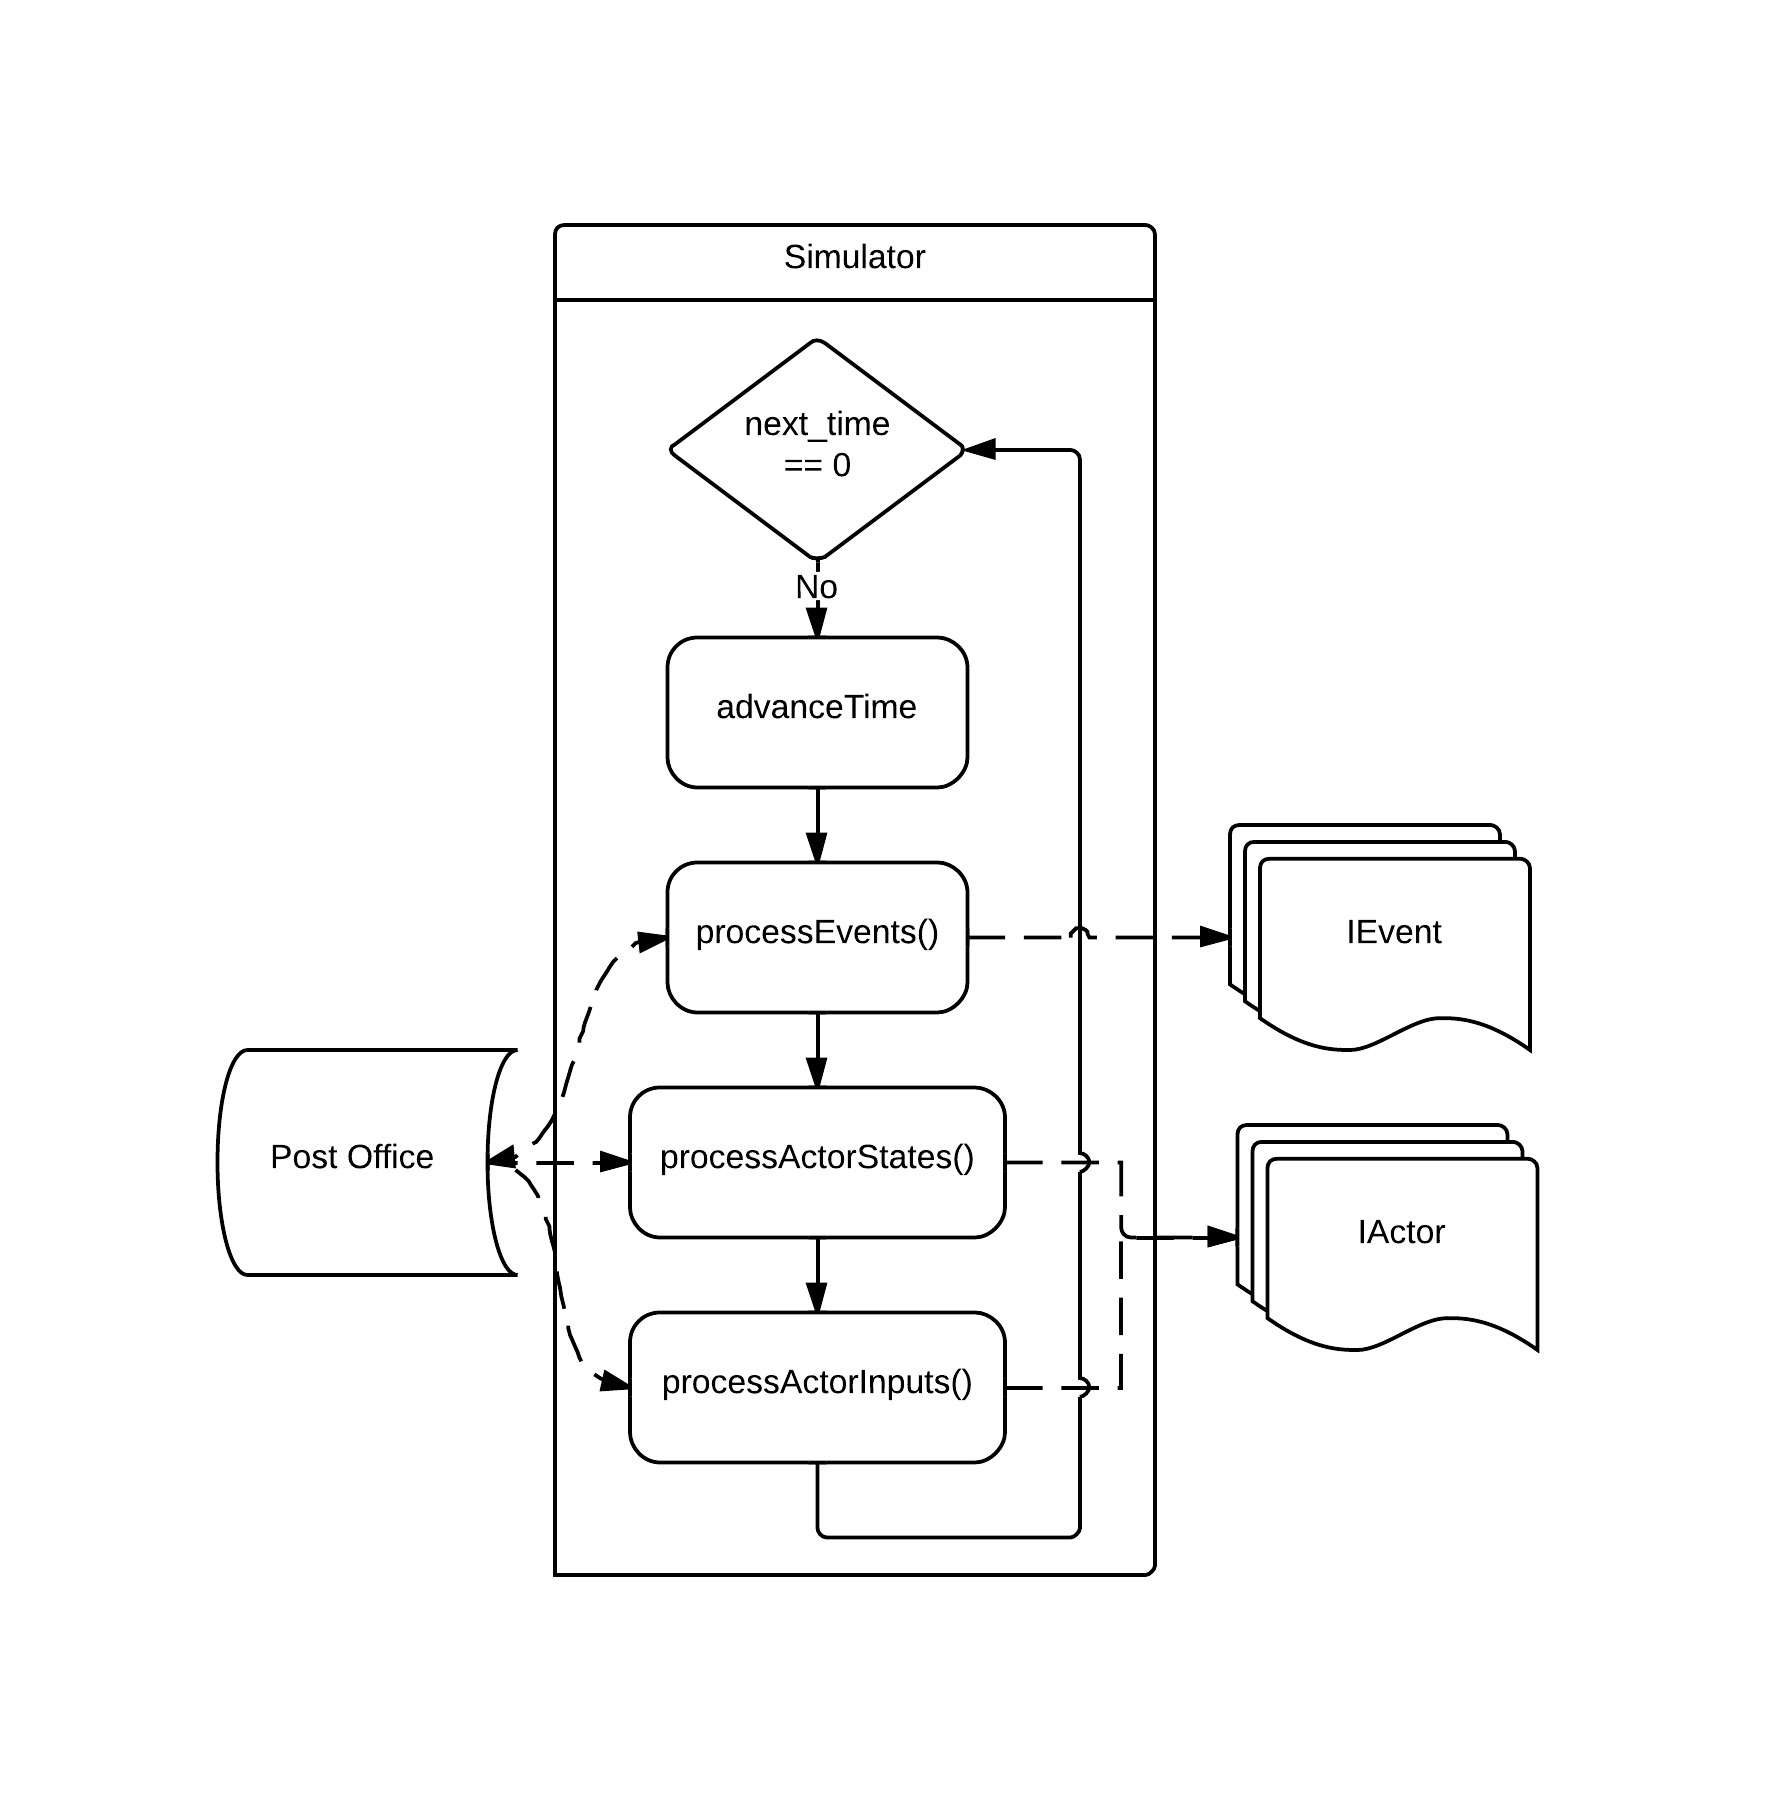
\includegraphics[width=2.5in, trim = 3in 3in 3in 3in, clip]{simulator.jpg}
\caption{Basic simulation timestep}
\label{simulator}
\end{figure}

Figure~\ref{simulator} portrays the execution of a time step. The simulator first processes the next state of any events that undergo a state change in that time. The outputs of those events are stored in the Post Office to be accessed by the Actors when applicable.  Next the simulator calls processInboundData on the PostOffice to move the temporary output to the current output. The Actors then each call processInputs.  Once each Actor has evaluated its inputs and made any changes the simulator checks if there are any future time-steps to evaluate and if not it terminates the simulation.

\subsection{Other Simulation Elements}

To help facilitate the simulation three other interfaces exist.  They are the ITeam, IData, and IState interfaces.  The ITeam interface acts as a wrapper around a team of Actors. The team represents all of the Actors that the simulator will interface with during the simulation and allows the simulator to call a single method on the team to perform actions on all of the Actors. The IData and IState interfaces are used to define common data types for passing information between Actors.  We use enumerations to define outputs and states specific to an Actor. These enumerations implement the correct interface for the type of information they carry.

\begin{verbatim}
public interface ITeam {
    public int getNextStateTime(int);
    public void processNextState();
    public void processInputs();
}

public interface IData {
    public String name();
}

public interface IState {
    public String name();
}
\end{verbatim}

The Simulator class provides a set of helper methods that are accessible to the Actors and Events.  We omit the list of these helper methods in the interest of space.

\begin{verbatim}
int getTime();
void setTime(int time);
int getNextStateTime();
void addOutput(String actor_name,
    IData input);
void addOutputs(String actor,
    ArrayList<IData> inputs);
ArrayList<IData> getInput(String actor);
void linkInput(String parent,
    String child);
void linkObservations(String parent,
    String child);
ArrayList<IData> getObservations(String);
void addObservation(IData data,
    String actor);
void addObservations(ArrayList<IData> data,
    String actor);
void addEvent(IEvent event);
int duration(Range range) ;
\end{verbatim}

This modeling framework imposes no other constraints on the model besides the simulation structure defined by these interfaces.  The model implementation has the full power of the Java language for all internal decision making.  We believe that this will ensure that the framework will be capable of simulating any and all aspects of the UAS model.  This contrasts with semantically constrained modeling languages such as Brahms that, due to the semantics, may not fully map to the model.

\end{comment}


\section{WiSAR UAS Model}
This section describes the models produced for the UAS-enabled WiSAR process.  We first discuss Actors and Events, followed by a brief discussion of Java asserts and a case study drawn from WiSAR.

This conceptual model uses Mealy state machines.  This allows us to abstract the different WiSAR roles into individual state machines that we call Actors.  Actor states do not correspond to a single aspect of the WiSAR domain, thus providing the freedom to flexibly model as many aspects of the domain as necessary and at various levels of resolution. Actors transition between states are triggered by inputs generated by Events and by other Actors.  Events are also modeled as Mealy machines whose transitions are triggered by a combination of simulator and Actor inputs. A benefit of this state machine-based conceptual model is the ability to convert the model into code. The coded model can be verified using model checking tools such as Java Pathfinder (JPF) to gain further insight into the model.  In the interest of space we will not describe the Java simulation framework developed for JPF model checking.

\subsection{Actors}
Choosing the core Actors is critical since modeling UAS-enabled WiSAR requires a level of abstraction that gives useful results without adding unnecessary complexity. After exploring several levels of abstraction, we selected a model that treats as an Actor any core decision-making element of the team, yielding the following Actors: parent search (PS), mission manager (MM), UAV operator (VeOp), video operator (VidOp), UAV operator GUI (VeGUI), video operator GUI (VidGUI), and the UAV.  We deliberately chose to not model ground searchers, leaving this to future work.

The models of the human roles use specific states for communication.  We describe these states once and then refer to them as a single communication state.  Typically before a human communicates he or she receives some signal that the communication is being received.  We model this as a POKE state.  When communicating, an Actor model of a human enters the POKE state where it waits until it receives an acknowledgement. If the acknowledgement is not received then the communication does not occur.  After the acknowledgement the human moves into a transmit (TX) state whose duration is based on the data being transferred.  At the end of this transfer the human enters an end (END) state and outputs the transferred data to the receiver. 

If the Actor model of the human receives a poke, then it responds with a busy or an acknowledge. If the human acknowledges the poke, then it enters the receive (RX) state. The human will not leave this state until the end communication input is received or until it decides to leave on its own. If one of these communications is interrupted before completion, then we consider that the data was not transferred. To better facilitate communication interruptions we only transfer a single piece of information per communication.

The next sections are dedicated to describing the Actor state machines with a generalized description of their relative transition matrixes.  We omit several of the previously mentioned Actors in the interest of space.

\begin{comment}
\begin{figure}
\center
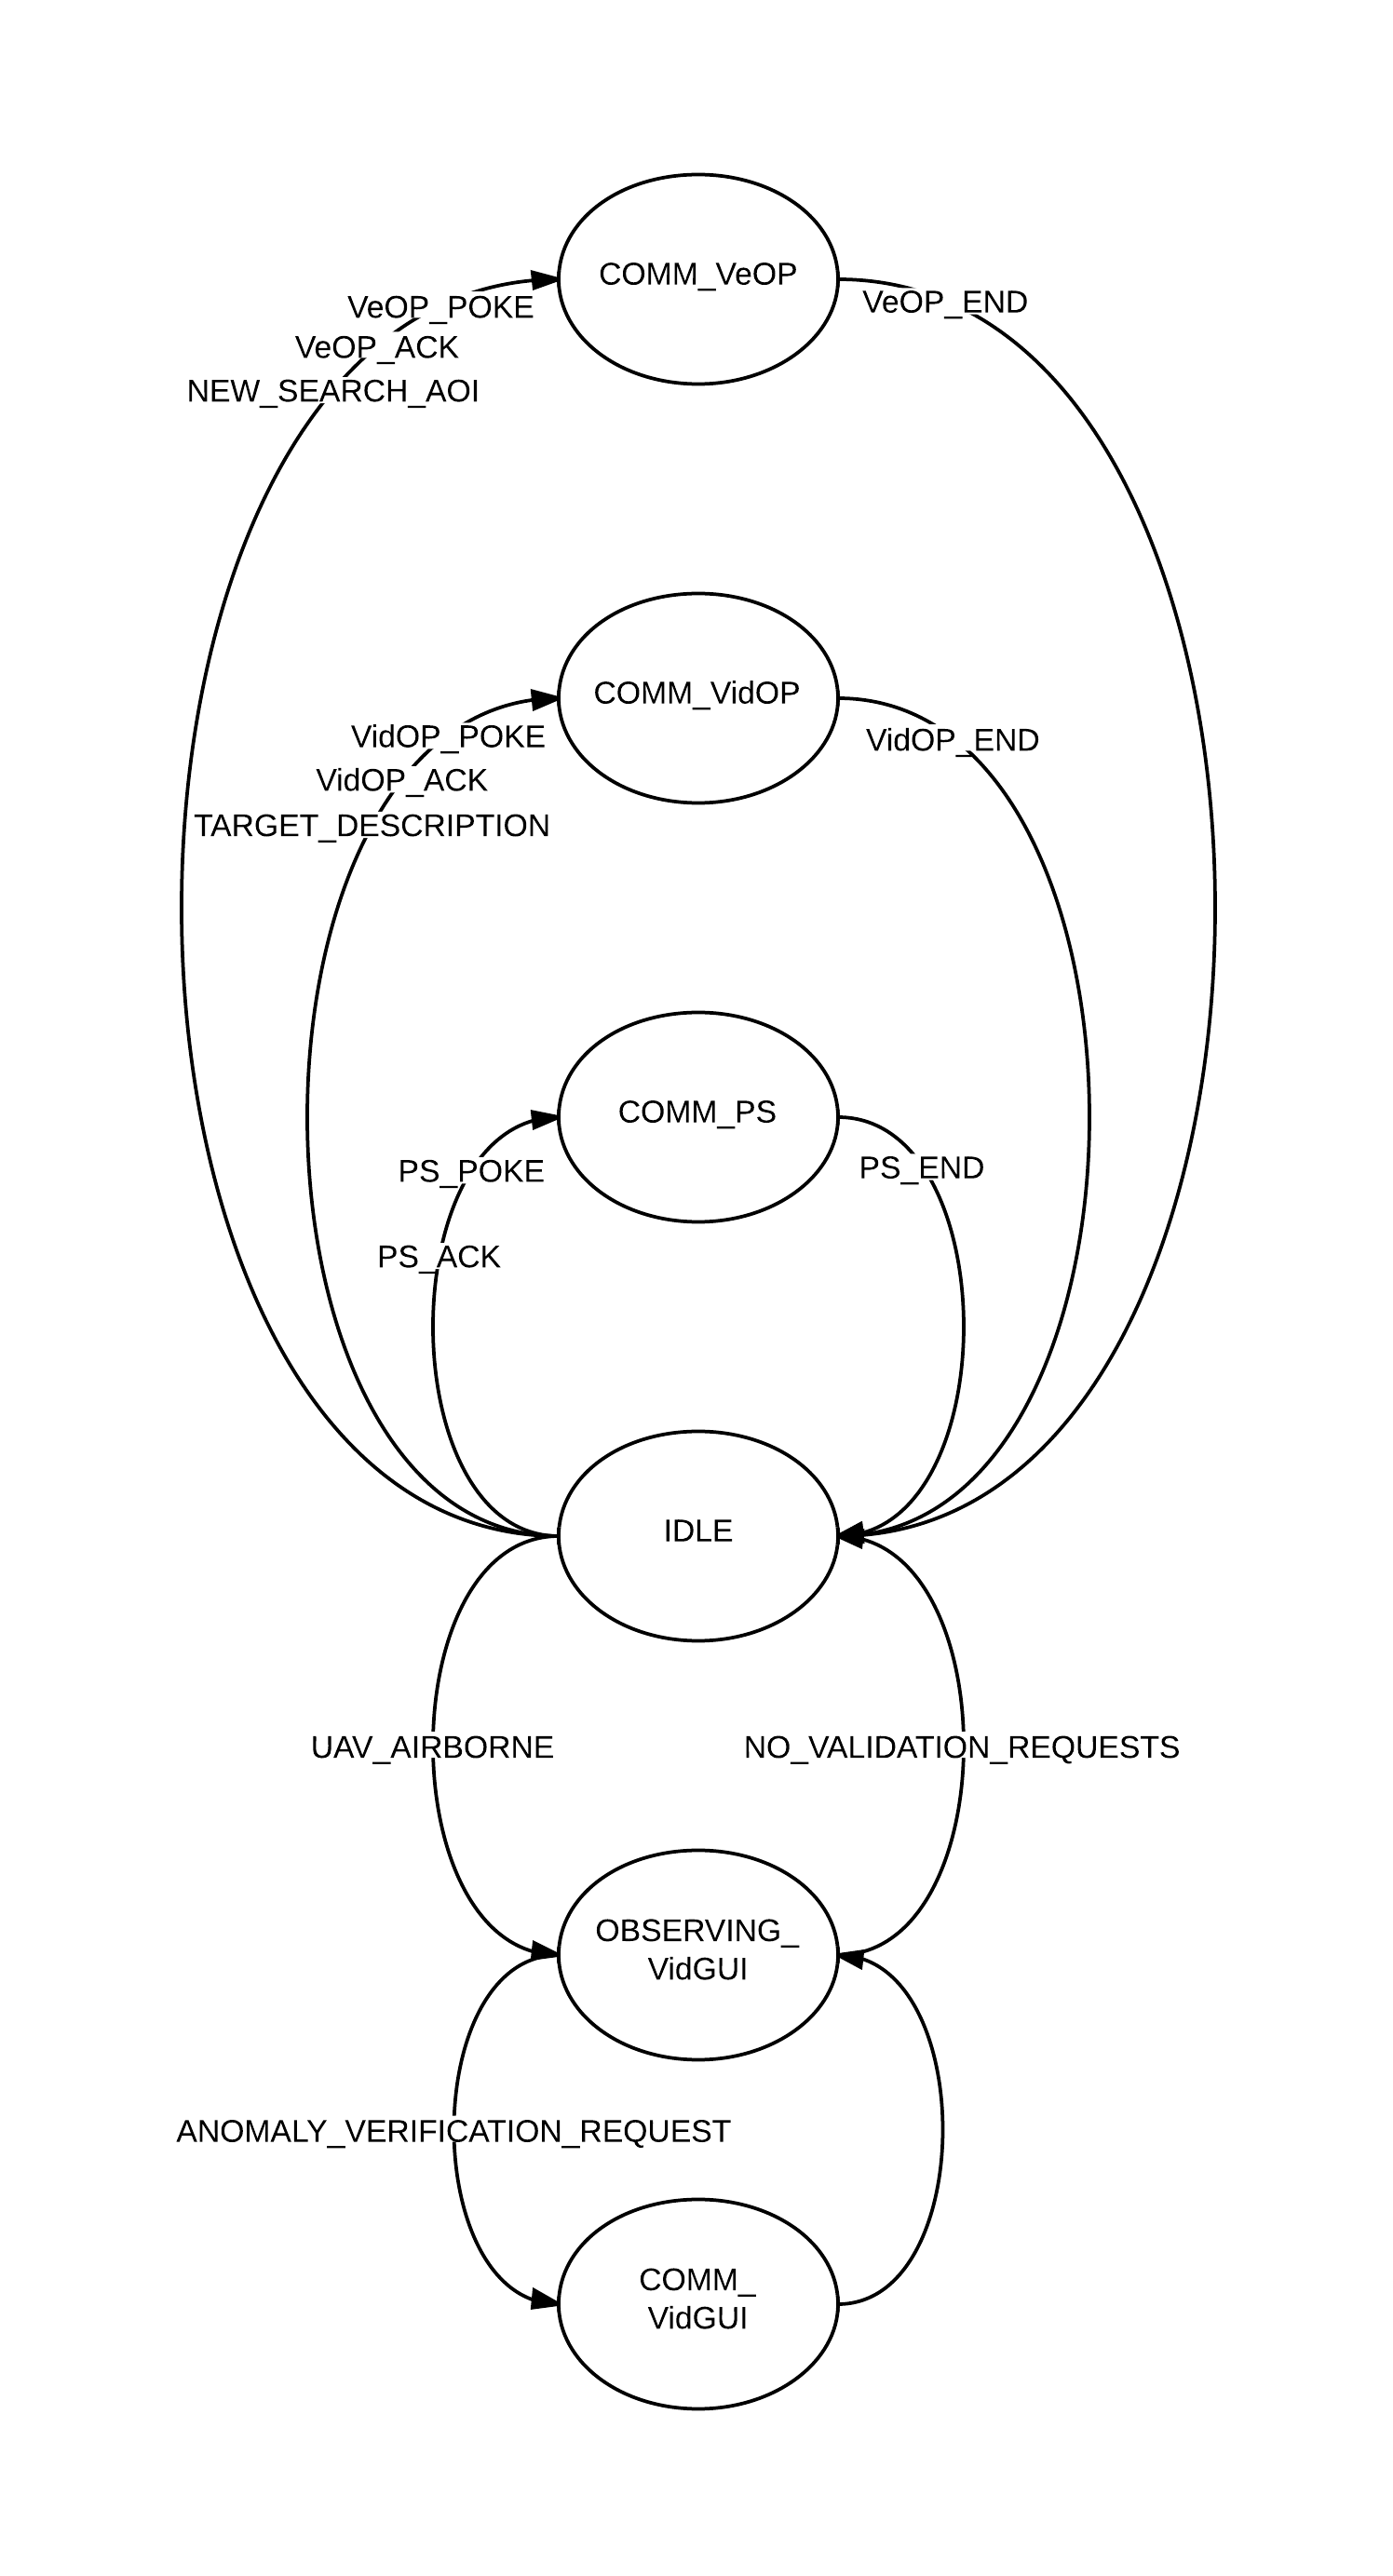
\includegraphics[width=3in]{mm_dirg.png}
\caption{Mission Manager DiRG. Excludes transition output.}
\label{fig:mmdirg}
\end{figure}
\end{comment}

\begin{figure}
\centering
\setlength{\abovecaptionskip}{1mm}
\setlength{\belowcaptionskip}{1mm}
\setlength{\textfloatsep}{1mm}
\setlength{\floatsep}{1mm}
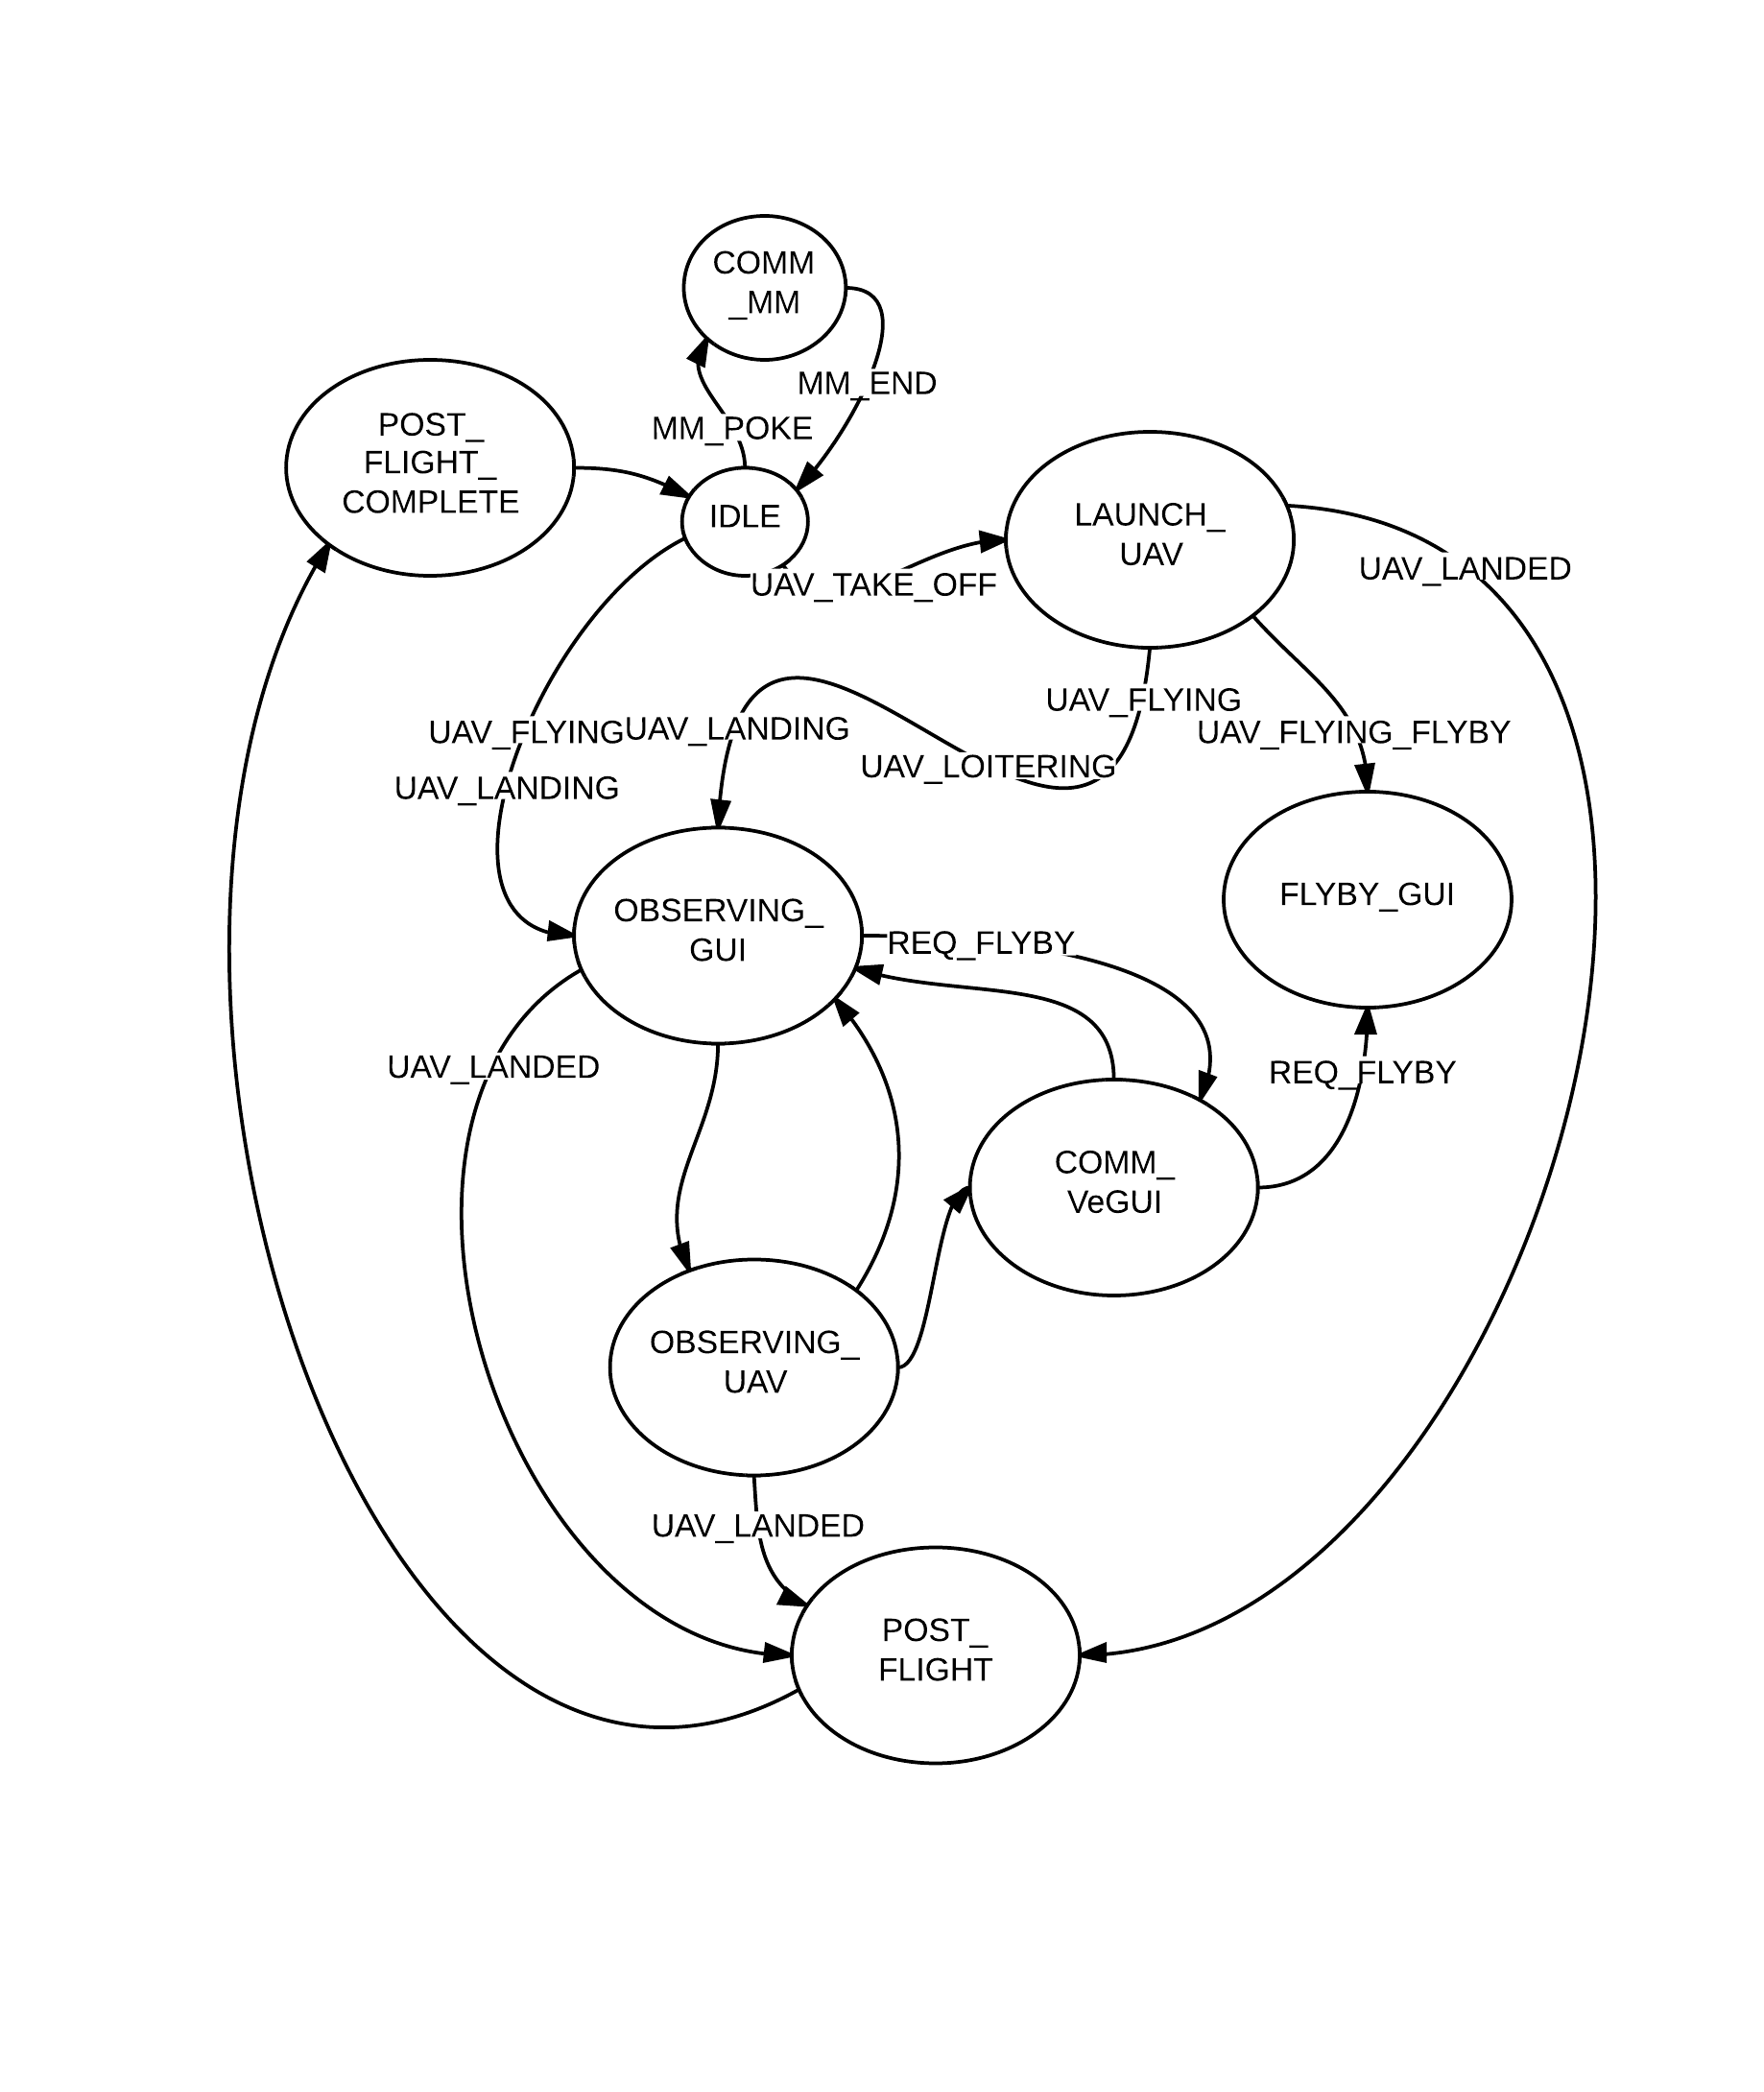
\includegraphics[width=3in, clip, trim=2.5in 4in 2.5in 3in, scale=2]{veop_dirg.png}
\caption{UAV Operator DiRG. Excludes transition output.}
\label{fig:veopdirg}
\end{figure}

\begin{figure}
\center
\setlength{\abovecaptionskip}{1mm}
\setlength{\belowcaptionskip}{1mm}
\setlength{\textfloatsep}{1mm}
\setlength{\floatsep}{1mm}
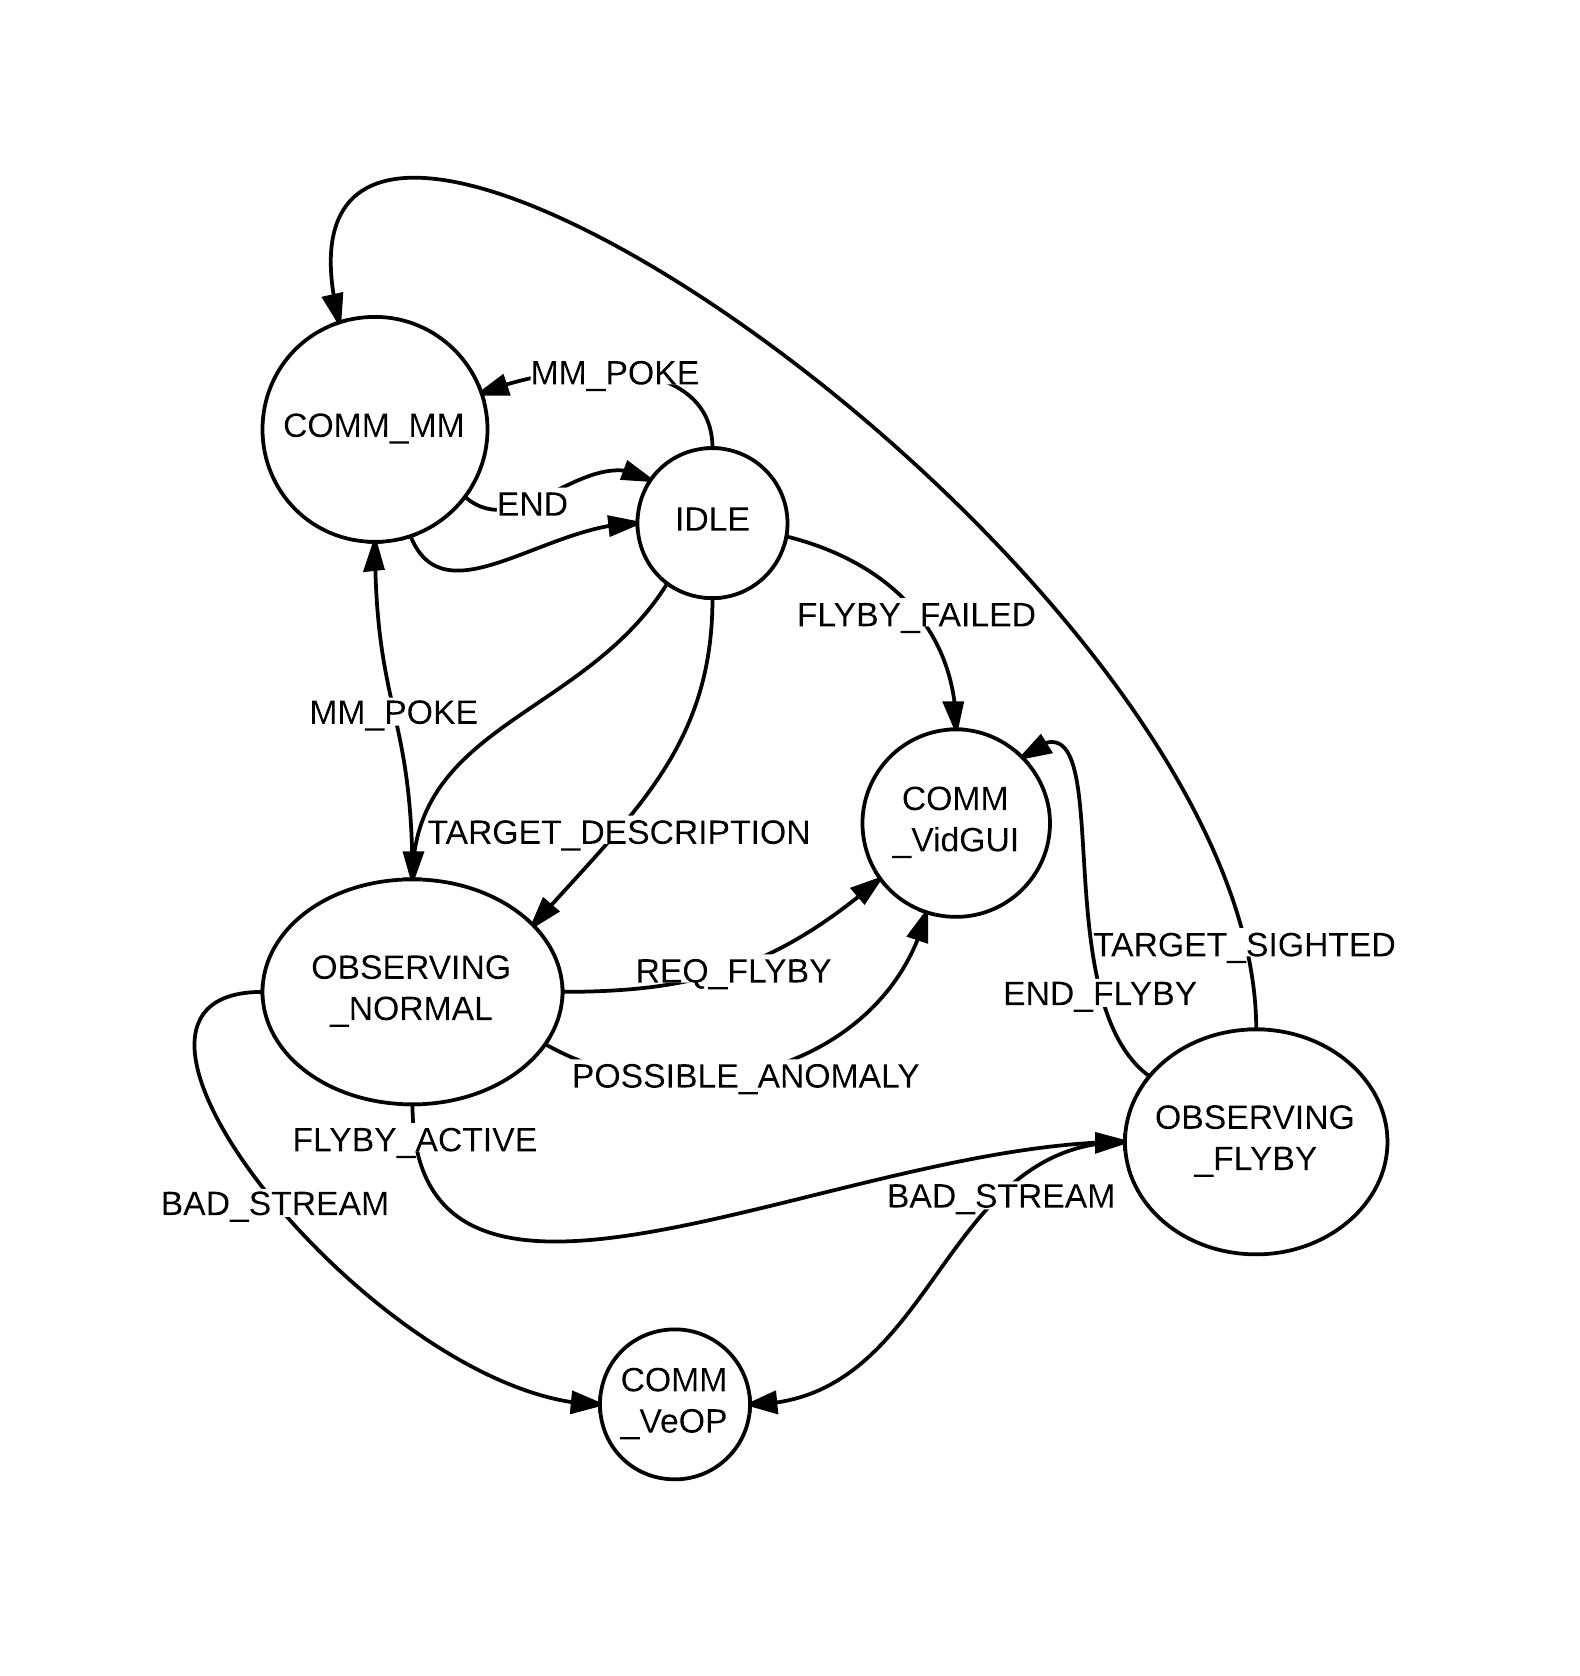
\includegraphics[height=3in, clip, trim=2in 2in 2in 2in]{vidop_dirg.png}
\caption{Video Operator DiRG. Excludes transition output.}
\label{fig:vidopdirg}
\end{figure}


% \subsubsection{Parent Search (PS)}
% This Actor loosely represents the incident commander but is heavily abstracted in our model.  The PS has two main states {\it IDLE} and communicating with the MM.  It contains no logic; it simply passes output from events to the MM and accepts input from the MM.  The events that it listens for are NewSearchAOIEvent, TargetDescriptionEvent, and TerminateSearchEvent described below.

% \subsubsection{Mission Manager (MM)}
% The MM Actor has the following states: {\it IDLE}, {\it OBSERVING\_VidGUI}, and three communication states: {\it PS}, {\it VeOp}, and {\it VidOp}.  Initially the MM is idle. After receiving a new search command and target description the MM distributes the received information. During the search the MM will periodically check the VidGUI to see if there are anomaly verification requests.  For each of these requests the MM will decide if it deserves a flyby or if it is a false positive.  While watching for anomaly verification requests the MM is also listening for input from the PS, VeOp, or VidOp.

\subsubsection{UAV Operator (VeOp)}
As illustrated in Figure~\ref{fig:veopdirg}, the VeOp Actor has the following states: {\it IDLE}, {\it OBSERVING\_VeGUI}, {\it FLYBY\_VeGUI}, {\it OBSERVING\_UAV}, {\it LAUNCH\_UAV}, {\it POST\_FLIGHT}, and three communication states: {\it MM}, {\it VeGUI}, and {\it VidOp}.  Initially the VeOp is idle.  After receiving a new search command from the MM the VeOp constructs a flight plan using the VeGUI.  When this is complete the VeOp will then launch the UAV.  While in the launch state the VeOp is observing the UAV, when the UAV completes its take off the VeOp moves to observing the VeGUI.  While the UAV is airborne the VeOp will continually move between observing the UAV and observing the VeGUI.  The VeOp will respond to any problems that are noticed while observing the VeGUI or UAV.

During the flight the VeOp listens for input from the PS and VidOp.  If there are flyby requests on the VeGUI, then the VeOp may choose to enter a flyby mode.  This implies a high cognitive load on the VeOp while positioning the UAV over the specified anomaly.  The VeOp will remain in flyby mode until the VidOp specifies, through the GUI, that the flyby is finished.  During an operation the UAV will often land and take off multiple times.  The post flight state represents the work necessary to get the UAV ready for flight, such as changing the battery.

\subsubsection{Video Operator (VidOp)}
As illustrated in Figue~\ref{fig:vidopdirg}, the VidOp Actor has the following states: {\it IDLE}, {\it OBSERVING\_VidGUI\_NORMAL},
{\it OBSERVING\_VidGUI\_FLYBY}, and three communication states: {\it MM}, {\it VeOp}, and {\it VidGUI}.  Initially the VidOp is idle.  After receiving a target description and the search information the VidOp moves to normal GUI observation.  While observing the VidGUI the VidOp watches for anomalies, each time an anomaly is visible the VidOp decides if the anomaly is seen.  If it is seen the VidOp decides if it is an unlikely, possible, or likely sighting.  This is done with probabilities related to the type of anomaly, true positive or false positive. If the anomaly is classified as possible then the VidOp makes a validate sighting request for the MM.  If the anomaly is a likely sighting then the VidOp requests a flyby from the VeOp. 

When the VeOp begins a flyby request the VidGUI signals the VidOp to enter the flyby state.  In this state the VidOp watches for the anomaly.  Due to the nature of the flyby the VidOp can now make an informed decision about the nature of the anomaly, gaining a much higher probability of being correct.  After deciding if it is the target the VidOp signals through the VidGUI that the flyby is finished.  If the sighting is confirmed the VidOp reports to the MM, otherwise the VidOp returns to normal GUI observation.

\subsubsection{Operator GUI (VeGUI)}
The VeGUI Actor has two states: {\it NORMAL} and {\it ALARM}. The VeGUI communicates directly with the UAV and VidGUI Actors. The default function of the VeGUI is to observe the UAV. The VeGUI keeps internal variables of all the UAV and VidGUI data that it tracks, all of this data is available through observation of the VeGUI.  If it detects an error with the UAV outputs such as low battery, no flight plan, low height above ground, or lost signal the VeGUI will enter the alarm state.  This state indicates that there are visible warnings on the screen to alert the VeOp of the problem.  The VeGUI listens for VeOp input or changes in the UAV output to signal that the problem has been dealt with before moving into the normal state.

% \subsubsection{Video Operator GUI (VidGUI)}
% The VidGUI Actor has two states: {\it NORMAL} and {\it FLYBY}.  The VidGUI has the same communication model as the VeGUI.  The default function of the VidGUI is to present anomalies to the VidOp.  The VidGUI presents anomalies by listening for input from TruePositiveAnomalyEvent and FalsePositiveAnomalyEvent.  The VidGUI tracks the visible anomalies, flyby requests, and anomaly verification requests.  The VidGUI moves to the flyby state after the VeOp initiates a flyby.  In this state the VidOp can observe that the UAV is attempting to relocate and obtain better video quality of a previously seen anomaly.  The VidGUI will remain in this state until it receives the finished command from the VidOp.  

\subsubsection{UAV}
The UAV Actor has the following states: {\it READY}, {\it TAKE\_OFF}, {\it FLYING}, {\it LOITERING},
{\it LANDING}, {\it LANDED} and {\it CRASHED}.  Initially the UAV is in the ready state.  Upon command the UAV moves to take off for a specific duration and then to flying or loitering.  The flying state is when the UAV is following a flight plan.  The loitering state is when the UAV is circling a specific location.  The UAV will automatically enter the loitering state after completing its flight plans.  While airborne the UAV, upon command, moves to the landing state for a specific duration before moving into the landed state.  Once landed the UAV must be moved into the ready state before it can take off again.

The Actors in this model, thus far, represent a fairly high level of abstraction.  Fortunately, the DiRG conceptual framework allows incremental extension of the models by adding lower levels of abstraction.  This is accomplished by introducing {\em sub-Actors} into the model.  We illustrate how the Actor/sub-Actor hierarchy can be used by describing two UAV sub-Actors.  In these examples the sub-Actors receive all the same input as the parent Actor and all sub-Actor output is sent from the parent Actor.

The first UAV sub-Actor is the UAVBattery. It contains the following states: {\it INACTIVE}, {\it ACTIVE}, {\it LOW}, and {\it DEAD}.  Initially the battery is inactive.  The battery is assigned a duration and a low battery threshold.  When the UAV receives the take off command the battery enters the active state.   The batteries next state is set to low at time $current\_time +  battery\_duration - low\_battery\_threshold$.  When the battery enters the low state its next state is set to dead at time $current\_time + low\_battery\_threshold$.

A second sub-Actor is the UAVFlightPlan. This represents the flight plan flown by the UAV. The flight plan requires a specific amount of time to complete.  The UAVFlightPlan has the following states: {\it NONE}, {\it ACTIVE}, {\it PAUSED}, and {\it COMPLETE}.  Initially the flight plan is set to none. After the operator creates a flight plan using the VeGUI then the flight plan moves to active.  During a flight the UAV may loiter, land, or flyby; this causes the flight plan to move to paused. When the UAV begins following the flight plan again it returns to active. After the UAV has flown the flight plan for the specified duration the flight plan enters the complete state.

The results discussed below include four other UAV sub-Actors: UAVHeightAboveGround, UAVSignal, UAVVidFeed, and FlybyAnomaly.  Details are omitted in the interest of space.

%The next sub-Actor is the UAVHeightAboveGround which has the following states: {\it INACTIVE}, {\it GOOD}, {\it LOW}, and {\it CRASHED}.  Its initial state is inactive..  This Actor represents the UAVs height above the ground (HAG).  Its main purpose is to listen for low height above ground events and to crash the UAV if a response is not received in time.  Once the UAV is airborne the HAG will remain good unless input is received from the LowHAGEvent.  The event moves the UAVHeightAboveGround into the low state.  If the UAV receives a modified flight plan then the state is changed back to good, otherwise the UAV will crash when it receives the second output from the LowHAGEvent..

%The next sub-Actor is the UAVSignal which has the folowing states: {\it OK} and {\it LOST}.  Initially it is set to OK.  This represents the UAVs communication with the VeGUI.  Its main purpose is to handle input from LostSignalEvent.  When this event occurs the signal enters the lost state until receiving input to return to the ok state.

%The next sub-Actor is the UAVVideoFeed which has the following states: {\it IDLE}, {\it OK} and {\it BAD}. This represents the quality of the UAV video feed.  Its purpose is to handle BadVideoFeedEvents. Its initial state is idle.  When the UAV takes off the video feed moves to OK.  When a BadVideoFeedEvent input is received the video feed moves to bad.  This is only returned to OK after the UAV has landed and taken off again.  Whenever the UAV is on the ground the state moves to idle.

%The last sub-Actor is the FlybyAnomaly which has the following states: {\it IDLE}, {\it ANOMALY\_NOT\_SEEN}, {\it ANOMALY\_SEEN}, {\it PAUSED}, and {\it FLYBY\_COMPLETE}.  This represents when the UAV is performing a flyby of a previously seen anomaly. Initially it is set to idle, indicating a flyby is not being executed. When a flyby is begun the FlybyAnomaly Actor moves into the anomaly not seen state for a specified duration before moving into the anomaly seen state, where it remains until the end flyby command is received.  During the anomaly seen state we assume that the anomaly is visible from the UAV and that it will remain visible until the flyby is complete.  When the end flyby command is received the FlybyAnomaly briefly enters the flyby complete state before returning back to idle.  If the UAV needs to land or loiter for any reason during the flyby it will enter a paused state.

\subsection{Events}
We used the Event Abstraction for several different elements of the UAS-enabled WiSAR problem. Adding this abstraction allows humans analyzing the system to give a set of inputs to the model and observe the consequences of the inputs.

\begin{comment}
Since all events behave similarly, despite the two classes of abstractions, we created a single state space that all Events use. Events have the following states:  {\it INACTIVE}, {\it ACTIVE}, and {\it FINISHED} (see figure~\ref{fig:eventdirg}). Initially all Events are inactive.  While inactive an Event will check to see if it is possible.  If the Event is possible then a timer is set to move the Event to active at some arbitrary future time; this allows Events to be triggered non-deterministically.  If the Event becomes impossible before becoming active the timer is removed.  Otherwise when it enters the active state its designated outputs are triggered and a timer is set for when it leaves the active state and enters the finished state.  At that point it outputs a signal indicating the event has terminated and returns to the inactive state. If there are multiple events, then it restarts the cycle until it has triggered a sufficient number of times.
 
\begin{figure}
\center
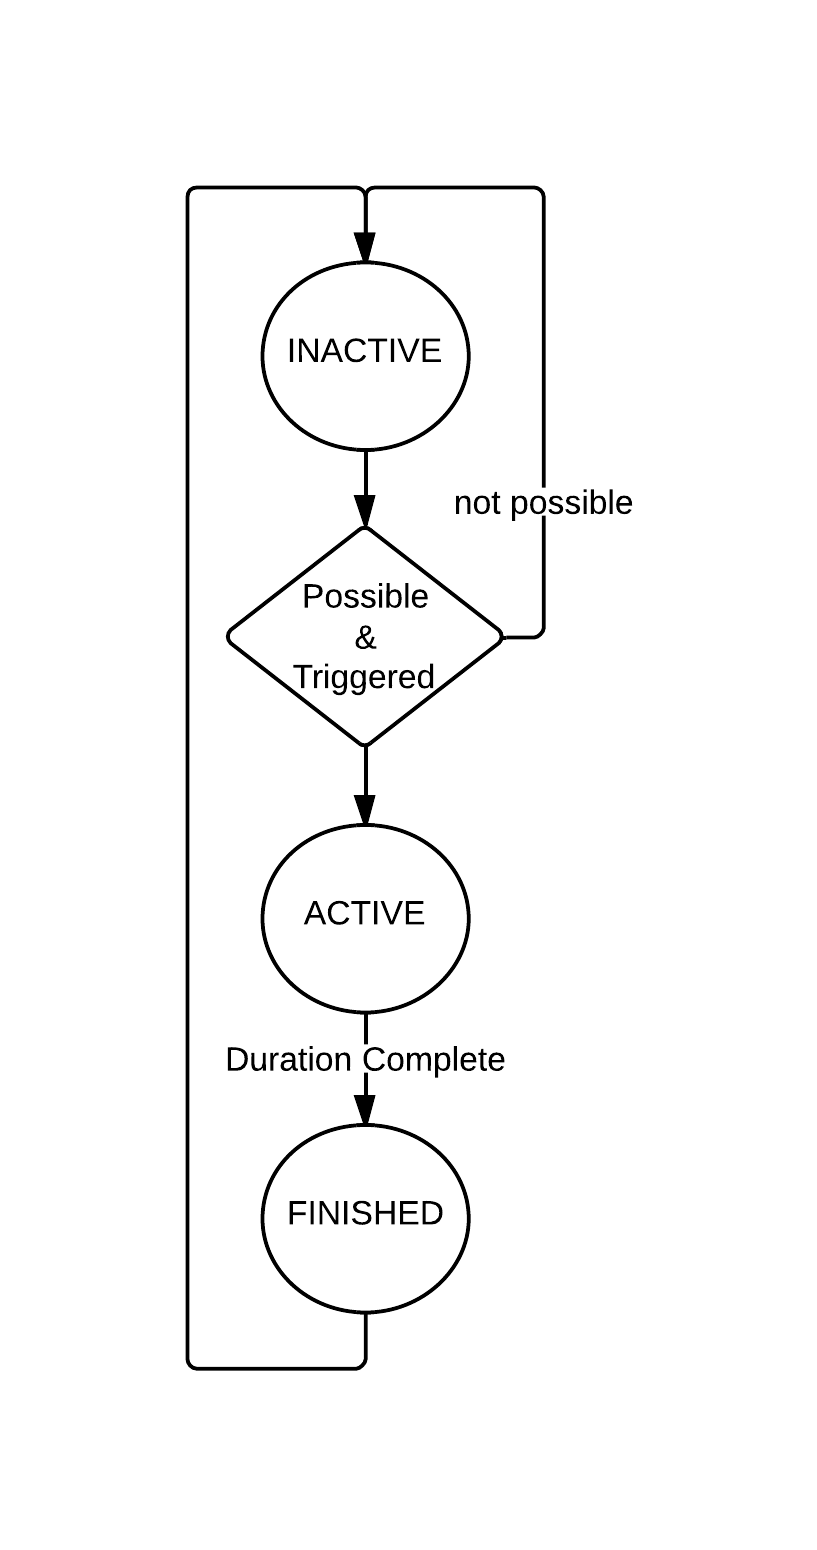
\includegraphics[width=2in]{event_dirg.png}
\caption{Event DiRG. Excludes transition output.}
\label{fig:eventdirg}
\end{figure} 
\end{comment}
The following Events were encountered in various UAS-enabled WiSAR field trials and represent a sample of interesting possible operating conditions for the Actors.  In the interest of space we list these events while omitting their descriptions.
NewSearchAOIEvent, TargetDescriptionEvent, TerminateSearchEvent, LowHAGEvent, LostSignalEvent, TruePositiveAnomalyEvent, FalsePositiveAnomalyEvent, and BadVideoFeedEvent.\footnote{HAG = Height Above Ground, AOI = Area of Interest}
\begin{comment}
\subsubsection{NewSearchAOIEvent}
This event outputs a new search area of interest (AOI) to the PS.  The VeOp cannot perform its duties until this output is received.
\subsubsection{TargetDescriptionEvent}
This event outputs a target description to the PS.  The VidOp cannot perform their duties until this output is received.
\subsubsection{TerminateSearchEvent}
This event outputs a terminate command to the PS.  The parent search may terminate for a multitude of reasons and at anytime.
\subsubsection{LowHAGEvent}
This event is only available while the UAV is airborne, it outputs height above ground(HAG) is low.  This event sends a second output after a specified period indicating that the UAV crashed.  This output is ignored if the flight plan was modified.
\subsubsection{LostSignalEvent}
This event is only available while the UAV is airborne.  It first sends a lost signal output.  After a specified duration it then sends an ok signal output.
\subsubsection{TruePositiveAnomalyEvent}
Only possible while the UAV is flying its flight plan.  Outputs an initial signal that the anomaly is visible.  Outputs a second signal that the anomaly is no longer visible.
\subsubsection{FalsePositiveAnomalyEvent}
Same process as TruePositiveAnomalyEvent.
\subsubsection{BadVideoFeedEvent}
Only available while the UAVVideoFeed is ok.  Outputs that the video quality is now too poor to be effective.
\end{comment}

\subsection{Asserts}
As a general rule in model-checking, the more complex the model the more that can go wrong. Detecting flaws in the model is extremely valuable because such flaws trigger further evaluation.  We present a case study in the next section that illustrates how the evaluation can identify things that need to change in the WiSAR process to avoid serious errors and perhaps failure to find the missing person.  

Unfortunately, it can be challenging to differentiate between important flaws and coding bugs.  To catch all errors, both flaws and bugs, we use Java Asserts. JPF automatically halts processing when it
encounters a false assertion, allowing us to determine if the error is a bug or
a flaw.

The model uses asserts in two ways. The first is detection of an
undesired state. If an actor enters an undesirable state then an assertion halts
the simulation. An example of this is the {\it UAV\_CRASHED} state. The second deals with inputs. Many operations are sequential.  They require a specific state and input before the next task can be performed. By looking at an Actors received inputs we are able to tell if an Actor is out of sync with the other Actors. An example of this
is the {\it VeOp\_TAKE\_OFF} input for the UAV. If the UAV is already airborne and it
receives this input we know that the operator is out of sync with the UAV.

Asserts are critical to debugging and verifying of the model.  We found that
having too many asserts is preferable to having too few.

\subsection{Case Study: Anomaly Detection}
The scenario illustrated in figure~\ref{state_machine} represents a portion of what should occur when the video operator believes a target has appeared on the video GUI. Each vertical swimlane represents an Actor/ DiRG.  Periodically during a flight the UAV will fly over an anomaly.  An anomaly can be either a false positive or a true positive,  meaning that it is either the desired target or it is not.  If the video operator believes that it is the target then a flyby request is made through the video GUI.  This request is then made visible to the operator through the operator GUI.  When the operator decides to perform the flyby request he signals this through the operator GUI and begins to manually direct the UAV to the location of the anomaly.  While the operator is directing the UAV the video operator closely examines the video stream until the anomaly is visible again.  The video operator then decides if it is a true target sighting or a false positive.  The video operator communicates this to the operator through the video GUI.  If it was a target sighting then the video operator passes the information to the mission manager who then passes it to the parent search. This high level view communicates the basic structure of the communication between the different actors.

\begin{figure}
\center
\setlength{\abovecaptionskip}{1mm}
\setlength{\belowcaptionskip}{1mm}
\setlength{\textfloatsep}{1mm}
\setlength{\floatsep}{1mm}
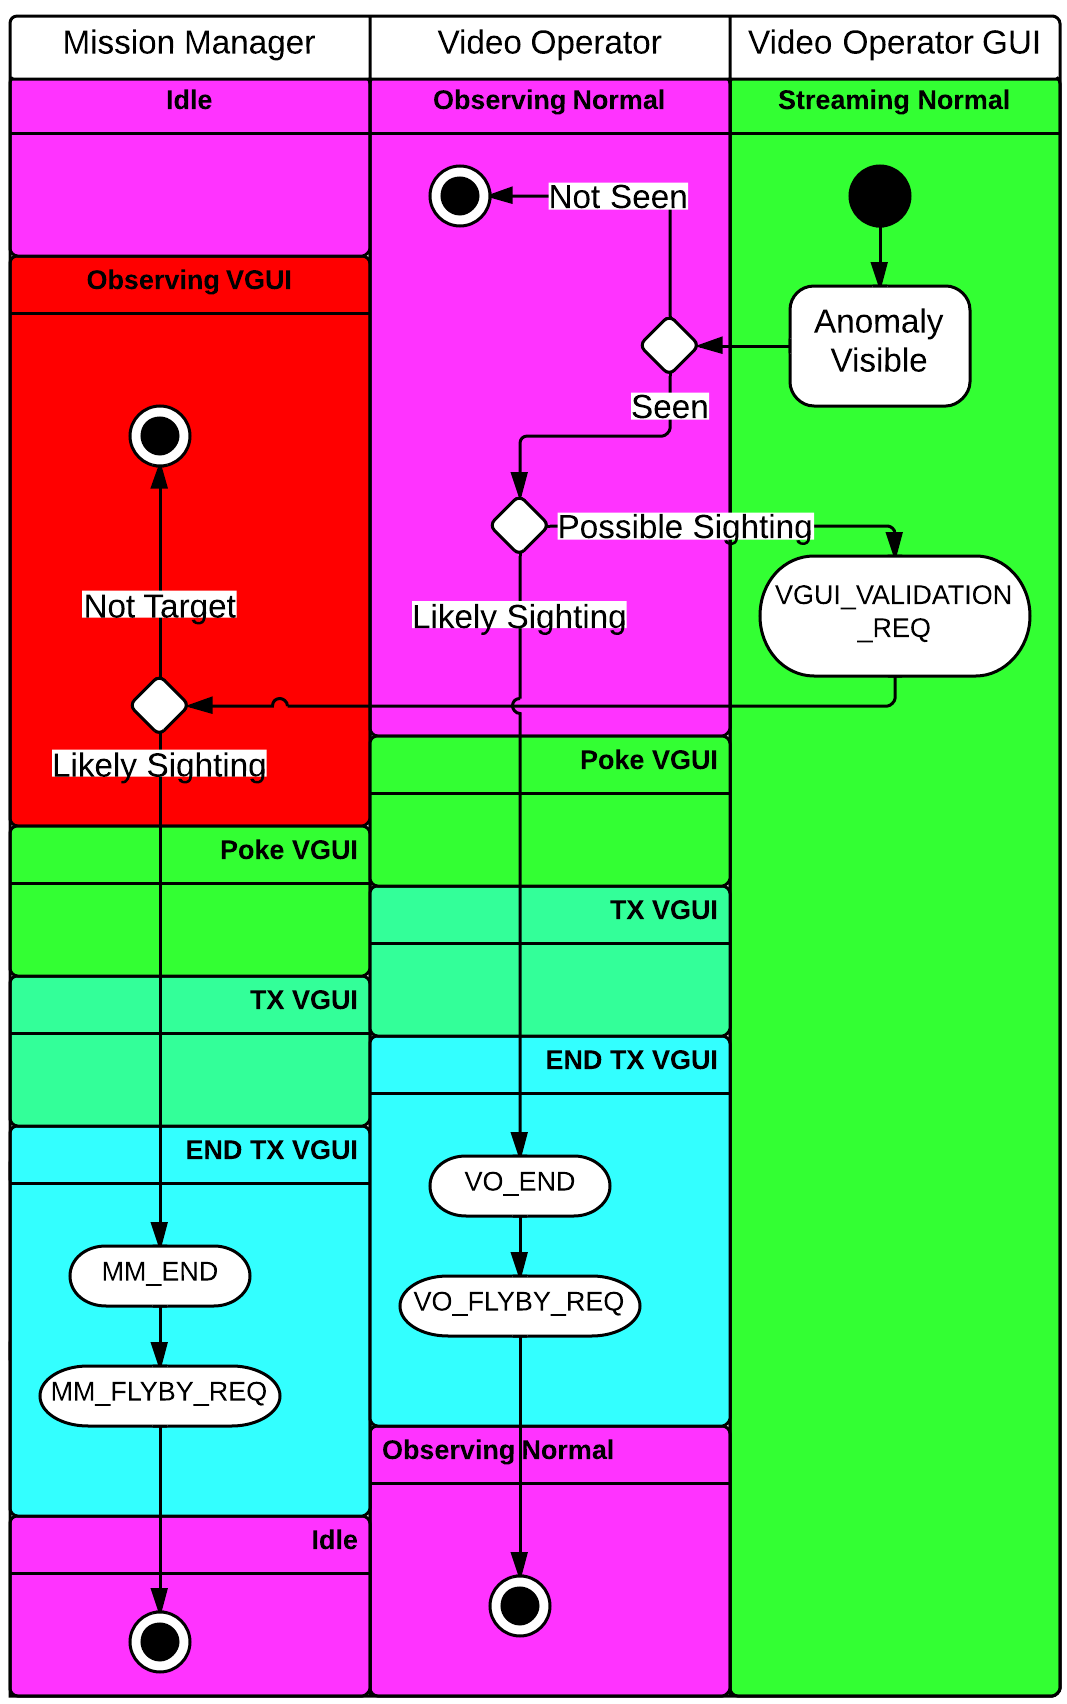
\includegraphics[width=\textwidth]{state_machine.png}
\caption{Anomaly Detection Model: Swim lanes represent actors.  Arrows
represent input/output.  Colored sections represent actor states.}
\label{state_machine}
\end{figure}


\section{Results}
%In this section we present empirical results to demonstrate that WiSAR UAS is
%modeled effectively using the approach we have taken.
%We will demonstrate this using a brief case study extracted from WiSAR UAS.  We
%will then give an analysis of the JPF results we obtained when we verified the
%model.

In this section, we first discuss model-checking results and then present insights from the modeling process.

%\subsection{Model Construction}
%As mentioned in section $V$ we use seven core actors in our model.  The anomaly detection effects each of these actors.  %Because we already had the core actor classes setup before we defined this part of the model it was a simple process of  %adding additional states and transitions to our actors.  For the anomalies themselves we created an anomaly event which sent %output directly to the video GUI.  We wanted the operator to non-deterministically choose if an anomaly was not seen, seen as %a possible target, or seen as a likely target.  We were able to achieve this by generating a random probability within a %designated range.  This means that when run by JPF each of those probabilities will be explored.  A small portion of the model %can be seen in
%figure~\ref{state_machine}.





\subsection{JPF Results}
Model checking constructs an exhaustive proof, by enumerating every reachable state of a system, to establish a property. The JPF model checker uses native Java as the modeling language to describe a system, and implements a custom virtual machine to systematically explore the reachable state space of the compiled Java program. The reachable state space of a sequential model is trivial to enumerate but the reachable state space grows exponentially with the level of non-determinism (i.e., random choice).

The source of non-determinism in the WiSAR model is in timing. The model defines time bounds for different events and tasks in the system. When the model is run, it non-deterministically chooses delays from within those bounds. For example, the time to land the UAV is a uniform random variable bounded between 60 and 1,800 time units. In the WiSAR model, there are 69 different tasks or events with non-deterministic durations. As it is not feasible to enumerate the entire reachable state space of such a large model, this work implements several standard heuristics to limit the non-determinism: minimum(maximum) time only;  minimum and maximum times only; and minimum, maximum, and mean times only. As expected, the first heuristic using only the minimum(maximum) time bound results in a sequential model with no non-determinism.

The total number of meaningful lines of code, code within methods, for the WiSAR model is 3,804. JPF is able to analyze the model using the minimum heuristic in negligible time only enumerating 124 states on a MacBook Air with 4GB of memory and an Intel Core I7 1.6 Ghz processor. The maximum heuristic also has negligible time but fewer behaviors with only 16 states. The difference in states is due to the UAV not needing to land several times to recharge its battery. 

The minimum and maximum bounds heuristic in JPF generates an important and interesting result. JPF finds a combination of task durations that result in an infinite loop using the heuristic. The same infinite loop can be recreated outside of JPF by repeatedly running the model over and over again as random trials until one of the trails goes into an infinite loop. The power of using JPF is that it finds the infinite loop every time without the need for the random trials. The root cause of the infinite loop was a flawed communication protocol that implicitly relied on specific delays in the interaction.  The protocol has since been corrected and JPF verifies the model to now terminate under all combinations of minimum or maximum delays: 3,911 states in 6 seconds of running time. 

The greatest number of states enumerated by JPF comes  from using the minimum, maximum, and mean heuristic. For all 69 points of non-determinism in the WiSAR model, JPF exhaustively considers 3 distinct values for each point, and checks every possible combination. JPF enumerates 51,344 states in around 52 seconds using the heuristic. None of the states violate the current set of assertions in the model and the model terminates under all the duration combinations. The jump in the number of states between the minimum and maximum bounds heuristic and this heuristic illustrates the exponential state explosion inherent in model checking. 

The JPF model checking does not prove the WiSAR model is the desired model or even a correct working model. There is considerable research yet to be completed in writing the system level requirements of WiSAR and then having JPF verify each of those requirements. If JPF finds a violation on any given requirement, there is still considerable work to determine if the requirement is correct (i.e., really what is desired from the system), if the model has a bug, or if the protocols in the model are fundamentally flawed and not able to implement the requirement. These topics are future work for the WiSAR model.

\begin{comment}
 In the context of the WiSAR model, model checking systematically enumerates every reachable state of the model in an effort to violate user defined assertions. 

The model contains 69 task duration ranges. A duration range defines a relative minimum and maximum time needed to complete a task.  Each time the model requests a duration the simulator non-deterministically returns a value from that range based on the simulation settings.  See Table~\ref{tab:jpf}.  JPF made it possible to explore the different paths created by the non-deterministic task durations.  

The entire Java code base consists of  $22,166$ lines of code which includes everything but spaces.  If looking at just lines of code within methods (LOCm), which represents the interface implementations, the number of key lines of code drops to $3804$.  See Table~\ref{tab:code}.   We ran our model checking on a MacBook Air with 4GB of memory and a 1.6Ghz Intel Core I7 processor.  With deterministic task durations we found a significant difference in the new states between the {\it MIN} and {\it MAX} durations.  When we increased the non-determinism, the number of new states exploded (see {\it MIN\_OR\_MAX} vs {\it MIN\_MEAN\_OR\_MAX}). See Table~\ref{tab:jpf}.  

These results were generated using a simplified version of our model, fewer Events and assertions, which runs to completion.  That is, a search area is received, the team searches the area finding nothing, and the PS is informed.  While the lack of assertions and other output makes it difficult to interpret these results they begin to show us how we can gain insight into WiSAR.  The difference between the number of new states between {\it MIN} and {\it MAX} durations tells us it takes more tasks to complete the same thing when task duration is lowered.  By using {\it MIN\_OR\_MAX} or {\it MIN\_MEAN\_OR\_MAX} JPF can automatically tell us which of those durations causes the greatest increase in new states.  In this particular scenario the minimum UAV battery duration forced the UAV to land several times to complete the same search.
\end{comment}

\begin{comment}
\begin{table*}
\begin{center}
\caption{metrics obtained using  the EclipseMetrics plugin}
\label{tab:code}
\begin{tabular}{ l || c c c c c c c c}
 & LINE & LOCm & CC & NOS & NLS & NOL & FE  NOP \\
\hline\\
Simulator & 5327 & 715 & 160 & 413 & 10 & 129 & 16 & 56 \\
Model & 16839 & 3089 & 740 & 2684 & 1 & 311 & 249 & 37 \\
Total & 22166 & 3804 & 900 & 3097 & 11 & 440 & 265 & 93 \\
\end{tabular}
\end{center}
\end{table*}
\end{comment}

\begin{comment}
There were a few cases when JPF would enter an infinite loop.  In two of these cases we found that we had an error in our model.  The first error occurred because an Actor was not receiving the input necessary to transition properly.  The second error occurred because we had an implicit transition instead of an explicit transition.  From this we learned the importance of expressing transitions explicitly and in validating the connectivity of the model which we plan to implement as future upgrades to our simulator.
\end{comment}

\subsection{Lessons from Modeling}
One of the goals of using model-checking with UAS-enabled WiSAR is to discover problems and opportunities with the structure of the organization.  This section presents several important lessons for UAS-enabled WiSAR that were obtained through the modeling exercise. 

First, while modeling the VidOp it became apparent that there was a problem with the organization.  This problem occurs because, while the VidOp is marking an anomaly, the video feed continues to run. This means that it is possible that the VidOp may miss detecting the target.  If the VidOp pauses the video, the feed falls behind the live video feed which makes flyby requests more expensive because the UAV will have to backtrack to the anomaly sighting.   We analyzed why this problem was not discovered in the WiSAR field trials.  The answer is that the field trials included multiple video feeds with multiple observers, a condition that is not likely to occur in a resource-limited search.  A lesson from this observation for WiSAR is that technology needs to be developed that allows the WiSAR team to manage this problem.  A more general lesson is that the modeling and model-checking process uncovered a potential problem before it appeared in practice.

A second lesson was learned when performing model-checking of a flyby.  Our model showed two problems, resuming a flight plan after a flyby and needing to keep a list of flyby requests.  We solved this in the model by adding visible queues to the VeGUI and VidGUI and allowing the VeGUI to store multiple flight plans.  As before, we analyzed why these problems were not discovered in the WiSAR field trials.  The answer is that these problems did occur but were not documented. The lesson for WiSAR is that the VeGUI and VidGUI need new features to support real searches.   A broader lesson is that the modeling exercise can be used to not only detect problems but specify the requirements for fixing them.

\begin{comment}
We add to these two specific lessons two meta-observations about creating an effectual process for modeling the system.  First, the exercise reminds us of the fact that verification is only as good as the questions asked.  Our initial success when the model ran to completion was tempered when we realized that it only implied that the code ran.  To obtain insight into specific aspects of the WiSAR UAS questions must first be described as assertions and outputs inside the model.

The second meta-observation is that the modeling approach needs to be able to be scalable to different levels of abstraction and different possible implementations of the system.  Through the modeling process, we can replace, change, and ignore processes or levels of detail.  This allows us to use scalable DiRGS to explore the ``what if's '' of the system instead of constraining ourselves to what currently happens with a system.
\end{comment}

\begin{comment}
\begin{table*}
\begin{center}
\caption{JPF results varied by the task duration}
\label{tab:jpf}
\begin{tabular}{ l || c  c  c  c c c}
Duration & Time & New & Visited & Backtracked & End & Max Depth \\
\hline \\
$MIN$ & 00:00:01 & 124 & 0 & 124 & 1 & 124 \\
$MAX$ & 00:00:00 & 16 & 0 & 16 & 1 & 16 \\
$MIN\_OR\_MAX$ & 00:00:06 & 3911 & 240 & 4151 & 72 & 129 \\
$MIN\_MEAN\_OR\_MAX$ & 00:00:52 & 51344 & 5193 & 56537 & 828 & 129 \\
\end{tabular}
\end{center}
\end{table*}
\end{comment}


%When we began to verify the model one of the first outputs we discovered was infinite loops.  This told us that something was %wrong. Typically this was caused by a failure to send the correct output, in one case an infinite loop occurred when the actor %would change states too early.  We discovered that the default maximum duration for that state was set too low.  This %represented a flaw in our model. 
%\subsection{Modeling Challenges}

%Another example was the addition of sub-actors to the UAV actor. Sub-actors are parts of a more complex actor, in this case %the UAV. The sub-actors of the UAV are the battery, flight plan, height above ground, and signal. Their inputs and
%outputs are handled differently than a normal actor. These sub-actor�s inputs are linked within the simulator to the UAV. The %UAV also has specific modifications that allow it to process all sub-actors before completing its own processing. This level of  %abstraction reduced the very complex UAV actor into multiple, simpler actors, which gave us confidence that this modeling %framework is robust enough to model anything we may need.  It also gave us a pattern for modeling the different levels of %abstraction that we desire.

%While constructing this portion of our model we used mock actors to represent some of the logic which belonged to the core %classes.  Mock actors are actor classes which always give the same output. This allowed us to get the model working before %we had finished coding. This proved to be very useful and we can see how it can be an effective tool for future verification.  If %we are not interested in the non-deterministic states of one actor, or a portion of that actors state space, that portion of the %model can be replaced with a mock actor.

%We did run into a few issues while coding the model.  One problem we found was inconsistency in our human memory %modeling.  Without a strict grammar it is possible to do the same thing in many different ways, which would lead
%to flaws in the model. We also found that if we did not move logic into sub-actors the complex actors began to be %unmanageably large.  In some cases moving logic into a sub-actor can be a difficult task.  Another problem we found was the %lack of asserts for invalid states and inputs.  These asserts are a crucial part of determining if the model is performing %correctly, but we had no way of enforcing that these asserts were placed into the code.

\section{Conclusions and Future Work}
%As stated previously this work is the basis for research on human machine interfaces that support combined human roles and %reduce operator workload.  To achieve this end we feel that the modeling framework we have presented would be
%more beneficial if it formalized some of the practices we found to be useful while modeling.  We would also like the simulation to %check the connectivity of the model before running the simulation to ensure that the transition matrix for each actor is complete.

We have presented DiRGs expressed as Mealy state machines for the purpose of modeling WiSAR in a way that will give insight into improving the WiSAR processes.  In addition we have coded these Mealy machines in Java and performed model-checking using the JPF tool for the purpose of gaining even more insight into our model by running it.  This contrasts with previous modeling attempts. Results show that additional insight was gained, and that it was possible to introduce new processes into the model and see the effect of those changes.

The result of the modeling and model checking processes was the detection of problems within WiSAR that were not seen during other analysis, or were seen but not documented.  The processes also gave insight, and in some cases specifications, for fixing the encountered problems.  

\begin{comment}
In the context of the future work outlined in the introduction, there are several important tasks that we feel will help us gain more insight into our model.  These are formal declarations of states, transitions, and task sequence verification built into the modeling framework.
\end{comment}

Future work will use explicit declarations to formalize Actor states and transition matrixes.  By formalizing these properties it will be possible to find transition errors immediately; it will also make it possible to compare the model with the model documentation for accuracy.  This may also make it possible to export the state machine into other model checkers.

We also plan to add sequential constraints to the model using Actors.  These Actor will embody the desired sequence of tasks and transitions and will throw assertions if a sequence is not executed in the desired order.  This will help us verify that the model is following the desired behaviors.

% conference papers do not normally have an appendix


% use section* for acknowledgement
\section*{Acknowledgment}
% optional entry into table of contents (if used)
% \addcontentsline{toc}{section}{Acknowledgment}
The authors would like to thank Neha Rungta of NASA Ames Intelligent
Systems Division for her help with JPF and Brahms. The authors would also like to thank the NSF IUCRC Center for Unmanned Aerial Systems, and the participating industries and labs, for funding the work. Further thanks go to Jared Moore and Robert Ivie for their help coding the model and editing this paper.








